	\documentclass[11pt,a4paper,notitlepage]{book}
\usepackage[utf8]{inputenc}
\usepackage[top=4cm,bottom=3cm]{geometry}
\usepackage{amsmath}
\usepackage{mathtools}
\usepackage{amssymb}
\usepackage{graphicx}
\usepackage{caption}
\usepackage[divpsnames]{xcolor}
\usepackage{subcaption}
%\usepackage{hyperref}
\usepackage[capitalise]{cleveref}
\usepackage{multirow}
\usepackage{aas_macros}
\usepackage{natbib, twoopt}
\usepackage{booktabs}
\usepackage{floatrow}
\newfloatcommand{capbtabbox}{table}[][\FBwidth]
\providecommand{\e}[1]{\ensuremath{\times 10^{#1}}}
\usepackage{listings}
%\lstset{language=C,
%  basicstyle=\footnotesize,
%  keywordstyle=\color{blue},
%  commentstyle=\color{green},
%  numberstyle=\color{magenta},
%  stringstyle=\color{blue},
%  identifierstyle=\color{black}
%}
\usepackage{color}
\usepackage{float}
\restylefloat{figure}
\usepackage{changepage}
\usepackage[titles]{tocloft}
\usepackage[justification=centering,font=small,labelsep=period,textfont=it,labelfont=bf]{caption}
\usepackage{url}
\usepackage{cleveref}
\newcommand{\Hrule}{\rule{\linewidth}{0.4mm}}
%\usepackage[french]{babel}
%\interfootnotelinepenalty=10000  % So that long footnotes bring their paragraph with them on next page
%\hypersetup{colorlinks=true,linkcolor=blue,citecolor=blue,urlcolor=cyan}

\bibpunct{}{}{;}{a}{}{,}
\newcommand{\HRule}{\rule{\linewidth}{0.5mm}}

\makeatletter
\newcommandtwoopt{\citeads}[3][][]{\href{http://adsabs.harvard.edu/abs/#3}%
{\def\hyper@linkstart##1##2{}%
\let\hyper@linkend\@empty\citealp[#1][#2]{#3}}}
\newcommandtwoopt{\citepads}[3][][]{\href{http://adsabs.harvard.edu/abs/#3}%
{\def\hyper@linkstart##1##2{}%
\let\hyper@linkend\@empty\citep[#1][#2]{#3}}}
\newcommandtwoopt{\citetads}[3][][]{\href{http://adsabs.harvard.edu/abs/#3}%
{\def\hyper@linkstart##1##2{}%
\let\hyper@linkend\@empty\citet[#1][#2]{#3}}}
\newcommandtwoopt{\citeyearads}[3][][]%
{\href{http://adsabs.harvard.edu/abs/#3}
{\def\hyper@linkstart##1##2{}%
\let\hyper@linkend\@empty\citeyear[#1][#2]{#3}}}
\makeatother


\usepackage{graphicx}
%\usepackage{psfig}
\usepackage{epstopdf}
\usepackage{cuted}
\usepackage{caption}
%\usepackage{draftwatermark}
\usepackage[bookmarks=false]{hyperref} %\usepackage{hyperref}
%\usepackage[capitalise]{cleveref}
%\usepackage{amssymb}
\usepackage{amsmath}
%\usepackage{aas_macros}
\usepackage{subcaption}
\usepackage{graphicx}
\usepackage{verbatim}
\usepackage{natbib}
\usepackage{rotate}
\usepackage{dsfont}
\usepackage{lscape}
%\usepackage{dsfont}
\usepackage{aalongtable}
\usepackage{supertabular}
\usepackage{mathbbol}
\usepackage{bm}
\usepackage{mathtools}
%\usepackage[subnum]{cases}
\usepackage{enumerate}
%\usepackage{draftcopy}
%\psdraft
%\usepackage[sc]{titlesec}
%\usepackage{bold-extra}
%\usepackage{arydshln}
\usepackage{amsmath}
%\usepackage{mathabx}
\usepackage{MnSymbol}
\allowdisplaybreaks
\usepackage{float}

\bibpunct{(}{)}{;}{a}{}{,}

\newcommand{\tbsp}{\rule{0pt}{18pt}}
\newcommand\sqdeg{deg$^{2}$}
\newcommand\psqdeg{deg$^{-2}$}
\newcommand\ugriz{u$^*$g'r'i'z'}
\newcommand\mic{$\mu$m}
\newcommand\AAn{\AA~}
\newcommand\sfr{SFR$_{0.5}$}
\newcommand\ssfr{sSFR$_{0.5}$}
\newcommand\msol{\mbox{M$_{\odot}$}}
\newcommand\wph{W.Hz$^{-1}$}
\newcommand\lsol{\mbox{L$_{\odot}$}}
\newcommand{\appropto}{\mathrel{\vcenter{
  \offinterlineskip\halign{\hfil$##$\cr
    \propto\cr\noalign{\kern2pt}\sim\cr\noalign{\kern-2pt}}}}}
%\usepackage{newtxtext,newtxmath}

\def\mathY{\bm{\mathcal{Y}}}
%\def\mathY{\bm{\mathcal{V}}}
\def\Bchi{\large\bm{\mathcal{\chi}}}
%\def\Bchi{\chi}
\def\PVec{\textbf{x}}
%% =======================
% === ETN definitions ===
% =======================

% paragraph macro
\def\pg{\paragraph{}}

% ++++++ variables ++++++
\def\evector{\textbf{\emph{e}}}
\def\Jones{\textbf{\emph{J}}}
\def\volt{\textbf{\emph{v}}}
\def\Vis{\textbf{V}}
\def\Herm{H}
\def\Bmatrix{\textbf{B}}
\def\U{\emph{\textbf{u}}}
\def\Kjones{\textbf{\emph{K}}}
\def\Gjones{\textbf{\emph{G}}}
\def\Ejones{\textbf{\emph{E}}}
\def\Wjones{\textbf{\emph{W}}}
\def\Coherency{\textbf{X}}
\def\direction{\pmb{\sigma}}
\def\lvec{\pmb{l}}
\def\uvec{\pmb{u}}


\def\Noisefunc{\mathcal{N}_{tt'}}
\def\Kfunc{\mathcal{K}_{tt'}}
\def\Errfunc#1{\mathcal{E}_{#1}}
\def\deltu{\delta u}
\def\deltv{\delta v}
\def\weight#1{\omega_{pq,#1}}
\def\deltasamp#1{\delta(#1-\underline{t}_0)}
\def\Sampfunc#1#2{\mathcal{C}_{#1}(#2)}
\def\DirFunc#1{\mathcal{S}_{#1}}
\def\WeightFunc#1{\mathcal{W}_{#1}}
\def\dudv{\delta u \delta v}
\def\t0{\mathbf{t_0}}



% operators
\def\Var#1{\textrm{Var}\{#1\}}
\def\Cov#1{\textrm{Cov}\{#1\}}
\def\Exp#1{\textrm{E}\{#1\}}
\def\Norm#1{\|#1\|}


% Algebra
\def\schur{\circ}

% Matrices
\def\matVt{\bm{\mathcal{V}}_t}
\def\matVdt{\bm{\mathcal{V}}_{d,t}}
\def\matKtd{\textbf{K}_{d,t}}
\def\matVV{\bigdoublevee}
\def\matR{\bm{R}}
\def\matRt{\bm{R}_t}
\def\matRdt{\bm{R}_{d,t}}

% Vectors
\def\vecktd{\textbf{k}_{d,t}}
\def\vecg{\vec{g}}
%\def\vecg{\textbf{g}}
\def\VecHatg{\widehat{\textbf{g}}}
\def\VecHatgt{\widehat{\textbf{g}_t}}
\def\VecHatgO{\widehat{\textbf{g}_{0}}}
\def\VarVecHatg{\textbf{V}_{\widehat{\textbf{g}}}}

% Scalars
\def\sqrts{\sqrt{s_d}}
\def\gpt{g_p^{t}}
\def\gqt{g_q^{t}}
\def\Hatgpt{\widehat{g_p^{t}}}
\def\Hatgqt{\widehat{g_q^{t}}}
\def\vpqt{v_{pq}^{t}}
\def\kpqdt{k_{pq,t}^{d}}
\def\kpdt{k_{p,t}^{d}}
\def\kqdt{k_{q,t}^{d}}
\def\kpqtlm{k^{lm}_{pq,t}}
\def\kpqtlmprime{k^{lm}_{pq,t'}}
\def\sd{s_{d}}
\def\Irpqlm{I^r_{pq,lm}}
\def\Vrpqt{\widetilde{r}_{pq,t}}
\def\Vrpqtprime{\widetilde{r}_{pq,t'}}


% ======= Names   =====================
\def\COH{{\sc CohJones}}

% ======= Scalars =====================
\def\u{u}
\def\v{v}
\def\w{w}
\def\l{l}
\def\m{m}
\def\n{n}
%\def\d{\text{d}}
\def\d{d}
\def\dbf{{\bm d}}


% ======= Conjugates
%\newcommand{\conj}[1]{{#1}^*}
%\newcommand{\conjp}[1]{{\left(#1\right)}^*}
\newcommand{\conj}[1]{\overline{#1}}
\newcommand{\conjp}[1]{\left({\overline{#1}}\right)}
%\newcommand{\Vec}[1]{\bm{#1}}
\def\vec#1{\ensuremath{\mathbf{#1}}}

% ======= 2x2 Matrices ===============
\def\JMat{\textbf{J}}
\def\Skyd{\textbf{S}_d}
\def\Vbl{\textbf{V}_{(pq)t\nu}}

\newcommand{\mat}[1]{{\bm{#1}}}
\newcommand{\JJ}{\mat{J}} % \bmath{\mathcal{J}}}
\newcommand{\JHJ}{\JJ^H\JJ} % \bmath{\mathcal{J}}}
\newcommand{\UL}{\mathrm{UL}}%\mathcal{ur}}
\newcommand{\Na}{N_\mathrm{ant}}
\newcommand{\Nbl}{N_\mathrm{bl}}
\newcommand{\Nd}{N_\mathrm{dir}}

% ======= Vectors      ===============
\def\vbltnu{\textbf{v}_{(pq)t\nu}}
\def\vbl{\textbf{v}_{pq}}
\def\V{\textbf{V}}
\def\gwirt{\bm{g_{\!_{W}}}}
\def\dgwirt{\dbf\bm{g_{\!_{W}}}}
\def\g{\bm{g}}
\def\vis{\textbf{v}}
\def\Vmeas{\textbf{P}}


% ====== Separator    ================
\def\separator{
\hrule
\begin{center}
\textsc{to be modified after that}
\end{center}
\hrule
}

% ======= Kroneker product ===========
\def\Kron{\otimes}

% ======= Jacobians =====================
\def\SimpleJacob{\bm{J}}
\def\Jacob{\bm{\mathcal{J}}}
%\def\JVpq{\Jacob\left\{\textbf{v}_{(pq)}\right\}}
%\def\JVpq{\Jacob_{\!_{\textbf{v}_{pq}}}}
\def\JVpq{\Jacob_{{\textbf{v}_{pq}},\bm{g_{\!_{W}}}}}
%\def\JVpq{\Jacob_{{\textbf{v}_{pq}}}}

\def\JVpqg{\Jacob_{{\textbf{v}_{pq}},\bm{g}}}
\def\JVpqCg{\Jacob_{{\textbf{v}_{pq}},\bm{\conj{g}}}}
%\def\JVpqg{\Jacob_{{\textbf{v}_{pq}}}\big|_{\bm{g}}}
%\def\JVpqCg{\Jacob_{{\textbf{v}_{pq}}}\big|_{\bm{\conj{g}}}}
\def\JVAtg{\JV\big|_{\vec{g}}}

\def\A{\textbf{A}}
\def\H{\textbf{H}}

\def\JV{\Jacob\left\{\textbf{v}\right\}}
%\def\JV{\Jacob_{\!_\textbf{v}}}
\def\JV{\Jacob_{\textbf{v}}}
%\def\JVpq{\Jacob_{\textbf{V}_{(pq)}}}
\def\JVg{\Jacob_{\textbf{v},\bm{g}}}
\def\JVCg{\Jacob_{\textbf{v},\bm{\conj{g}}}}

\newcommand{\FigDir}{../Figures/}


\def\supertiny{ \font\supertinyfont = cmr10 at 4pt \relax \supertinyfont}








\author{Etienne Bonnassieux}
\title{PhD manuscript}

% +++ IMPORT DEFINITIONS +++
% =======================
% === ETN definitions ===
% =======================

% paragraph macro
\def\pg{\paragraph{}}

% ++++++ variables ++++++
\def\evector{\textbf{\emph{e}}}
\def\Jones{\textbf{\emph{J}}}
\def\volt{\textbf{\emph{v}}}
\def\Vis{\textbf{V}}
\def\Herm{H}
\def\Bmatrix{\textbf{B}}
\def\U{\emph{\textbf{u}}}
\def\Kjones{\textbf{\emph{K}}}
\def\Gjones{\textbf{\emph{G}}}
\def\Ejones{\textbf{\emph{E}}}
\def\Wjones{\textbf{\emph{W}}}
\def\Coherency{\textbf{X}}
\def\direction{\pmb{\sigma}}
\def\lvec{\pmb{l}}
\def\uvec{\pmb{u}}


\def\Noisefunc{\mathcal{N}_{tt'}}
\def\Kfunc{\mathcal{K}_{tt'}}
\def\Errfunc#1{\mathcal{E}_{#1}}
\def\deltu{\delta u}
\def\deltv{\delta v}
\def\weight#1{\omega_{pq,#1}}
\def\deltasamp#1{\delta(#1-\underline{t}_0)}
\def\Sampfunc#1#2{\mathcal{C}_{#1}(#2)}
\def\DirFunc#1{\mathcal{S}_{#1}}
\def\WeightFunc#1{\mathcal{W}_{#1}}
\def\dudv{\delta u \delta v}
\def\t0{\mathbf{t_0}}



% operators
\def\Var#1{\textrm{Var}\{#1\}}
\def\Cov#1{\textrm{Cov}\{#1\}}
\def\Exp#1{\textrm{E}\{#1\}}
\def\Norm#1{\|#1\|}


% Algebra
\def\schur{\circ}

% Matrices
\def\matVt{\bm{\mathcal{V}}_t}
\def\matVdt{\bm{\mathcal{V}}_{d,t}}
\def\matKtd{\textbf{K}_{d,t}}
\def\matVV{\bigdoublevee}
\def\matR{\bm{R}}
\def\matRt{\bm{R}_t}
\def\matRdt{\bm{R}_{d,t}}

% Vectors
\def\vecktd{\textbf{k}_{d,t}}
\def\vecg{\vec{g}}
%\def\vecg{\textbf{g}}
\def\VecHatg{\widehat{\textbf{g}}}
\def\VecHatgt{\widehat{\textbf{g}_t}}
\def\VecHatgO{\widehat{\textbf{g}_{0}}}
\def\VarVecHatg{\textbf{V}_{\widehat{\textbf{g}}}}

% Scalars
\def\sqrts{\sqrt{s_d}}
\def\gpt{g_p^{t}}
\def\gqt{g_q^{t}}
\def\Hatgpt{\widehat{g_p^{t}}}
\def\Hatgqt{\widehat{g_q^{t}}}
\def\vpqt{v_{pq}^{t}}
\def\kpqdt{k_{pq,t}^{d}}
\def\kpdt{k_{p,t}^{d}}
\def\kqdt{k_{q,t}^{d}}
\def\kpqtlm{k^{lm}_{pq,t}}
\def\kpqtlmprime{k^{lm}_{pq,t'}}
\def\sd{s_{d}}
\def\Irpqlm{I^r_{pq,lm}}
\def\Vrpqt{\widetilde{r}_{pq,t}}
\def\Vrpqtprime{\widetilde{r}_{pq,t'}}


% ======= Names   =====================
\def\COH{{\sc CohJones}}

% ======= Scalars =====================
\def\u{u}
\def\v{v}
\def\w{w}
\def\l{l}
\def\m{m}
\def\n{n}
%\def\d{\text{d}}
\def\d{d}
\def\dbf{{\bm d}}


% ======= Conjugates
%\newcommand{\conj}[1]{{#1}^*}
%\newcommand{\conjp}[1]{{\left(#1\right)}^*}
\newcommand{\conj}[1]{\overline{#1}}
\newcommand{\conjp}[1]{\left({\overline{#1}}\right)}
%\newcommand{\Vec}[1]{\bm{#1}}
\def\vec#1{\ensuremath{\mathbf{#1}}}

% ======= 2x2 Matrices ===============
\def\JMat{\textbf{J}}
\def\Skyd{\textbf{S}_d}
\def\Vbl{\textbf{V}_{(pq)t\nu}}

\newcommand{\mat}[1]{{\bm{#1}}}
\newcommand{\JJ}{\mat{J}} % \bmath{\mathcal{J}}}
\newcommand{\JHJ}{\JJ^H\JJ} % \bmath{\mathcal{J}}}
\newcommand{\UL}{\mathrm{UL}}%\mathcal{ur}}
\newcommand{\Na}{N_\mathrm{ant}}
\newcommand{\Nbl}{N_\mathrm{bl}}
\newcommand{\Nd}{N_\mathrm{dir}}

% ======= Vectors      ===============
\def\vbltnu{\textbf{v}_{(pq)t\nu}}
\def\vbl{\textbf{v}_{pq}}
\def\V{\textbf{V}}
\def\gwirt{\bm{g_{\!_{W}}}}
\def\dgwirt{\dbf\bm{g_{\!_{W}}}}
\def\g{\bm{g}}
\def\vis{\textbf{v}}
\def\Vmeas{\textbf{P}}


% ====== Separator    ================
\def\separator{
\hrule
\begin{center}
\textsc{to be modified after that}
\end{center}
\hrule
}

% ======= Kroneker product ===========
\def\Kron{\otimes}

% ======= Jacobians =====================
\def\SimpleJacob{\bm{J}}
\def\Jacob{\bm{\mathcal{J}}}
%\def\JVpq{\Jacob\left\{\textbf{v}_{(pq)}\right\}}
%\def\JVpq{\Jacob_{\!_{\textbf{v}_{pq}}}}
\def\JVpq{\Jacob_{{\textbf{v}_{pq}},\bm{g_{\!_{W}}}}}
%\def\JVpq{\Jacob_{{\textbf{v}_{pq}}}}

\def\JVpqg{\Jacob_{{\textbf{v}_{pq}},\bm{g}}}
\def\JVpqCg{\Jacob_{{\textbf{v}_{pq}},\bm{\conj{g}}}}
%\def\JVpqg{\Jacob_{{\textbf{v}_{pq}}}\big|_{\bm{g}}}
%\def\JVpqCg{\Jacob_{{\textbf{v}_{pq}}}\big|_{\bm{\conj{g}}}}
\def\JVAtg{\JV\big|_{\vec{g}}}

\def\A{\textbf{A}}
\def\H{\textbf{H}}

\def\JV{\Jacob\left\{\textbf{v}\right\}}
%\def\JV{\Jacob_{\!_\textbf{v}}}
\def\JV{\Jacob_{\textbf{v}}}
%\def\JVpq{\Jacob_{\textbf{V}_{(pq)}}}
\def\JVg{\Jacob_{\textbf{v},\bm{g}}}
\def\JVCg{\Jacob_{\textbf{v},\bm{\conj{g}}}}



\begin{document}
%%%%%%%%%%%%%%%
%%% PREFACE %%%
%%%%%%%%%%%%%%%
\pagenumbering{roman}
%\newgeometry{top=1cm,bottom=1cm}

\begin{figure}[h]
\centering
\begin{minipage}{.45\textwidth}
\centering

\includegraphics[height=1.5cm]{titlepage/logo-psl.png}
\end{minipage}
\begin{minipage}{.45\textwidth}
\centering

\includegraphics[height=2.0cm]{titlepage/ska-logo.jpg}
\end{minipage}
\end{figure}
\vspace{1cm}
{\let\newpage\relax\maketitle}
\maketitle
\begin{center}
\Large{Supervisors: Philippe Zarka, Oleg Smirnov, Cyril Tasse}
\end{center}
\noindent\Hrule
\begin{center}
\Large{\underline{Title}}\\
\pg
title goes here
\end{center}
%\pg
Lorem ipsum dolor sit amet, consectetur adipiscing elit. Morbi vehicula dui vel sem elementum viverra. Nullam molestie egestas finibus. Vestibulum at rhoncus massa, ac mollis nulla. Nam vitae vestibulum ex. Interdum et malesuada fames ac ante ipsum primis in faucibus. Curabitur lobortis quam eget dui pretium pulvinar. Quisque consequat dapibus justo, eu blandit lacus auctor id. Vivamus vestibulum diam id feugiat posuere. Morbi ut vehicula urna, id laoreet turpis. Nam dignissim magna augue, et rhoncus felis lacinia nec. Praesent convallis ultrices hendrerit.

\pg
Praesent porta lacus est. Duis tempor augue augue, ac pharetra nisi viverra sed. Integer tristique risus ac metus aliquam, in pretium felis porttitor. Sed eu ipsum vitae tortor faucibus ultrices. Cras sem erat, eleifend eget massa et, dapibus vulputate velit. Duis semper non odio in semper. Mauris quis massa rhoncus ante ullamcorper faucibus. Nam quis sollicitudin diam. Maecenas et posuere augue, ac aliquam sapien. Curabitur ac tristique ante. Sed tempor tellus a magna vehicula fringilla. Suspendisse arcu lacus, bibendum vitae velit vel, posuere commodo ipsum. Suspendisse et congue sem. Maecenas maximus quam sed interdum dignissim. Etiam ac tempor risus. Quisque vel nisi arcu. Nunc consectetur, nisl nec blandit egestas, dolor felis tincidunt odio, et iaculis lacus nunc in sem. Suspendisse potenti. Aenean est ante, egestas ac nulla eu, suscipit maximus orci. Etiam suscipit neque sed diam hendrerit, eu iaculis risus laoreet. Sed venenatis ultricies justo porta placerat. Quisque ac convallis nunc. Suspendisse et risus enim.

\pg
Integer eu suscipit sem. Cras vestibulum felis sed hendrerit aliquet. Suspendisse consectetur cursus ex, nec mattis massa. Sed nec lacinia nunc, tristique suscipit ipsum. Suspendisse consectetur finibus erat, ac lobortis nisi bibendum sed. Praesent dictum dolor augue, eu aliquam ipsum facilisis ac. Proin consectetur massa et nisl porttitor, sit amet blandit risus egestas. Proin vestibulum odio ultrices nulla iaculis molestie. Nulla ut accumsan odio. Donec pellentesque non velit sed pharetra.
~\\
\Hrule
\vspace{2.5cm}
\begin{figure}[h]
\centering
\begin{minipage}{.45\textwidth}
\centering

\includegraphics[height=1.5cm]{titlepage/LogoLESIA.jpg}
\end{minipage}
%\begin{minipage}{.32\textwidth}
%\centering
%
\includegraphics[height=1.5cm]{titlepage/ens.png}
%\end{minipage}
\begin{minipage}{.45\textwidth}
\centering

\includegraphics[height=1.0cm]{titlepage/ratt-logo.png}
\end{minipage}
\end{figure}
\thispagestyle{empty}
\restoregeometry


\newpage
\setcounter{page}{1}
\tableofcontents

\newpage
\addtocontents{toc}{~\hfill\textbf{Page}\par}
%\pg
Lorem ipsum dolor sit amet, consectetur adipiscing elit. Morbi vehicula dui vel sem elementum viverra. Nullam molestie egestas finibus. Vestibulum at rhoncus massa, ac mollis nulla. Nam vitae vestibulum ex. Interdum et malesuada fames ac ante ipsum primis in faucibus. Curabitur lobortis quam eget dui pretium pulvinar. Quisque consequat dapibus justo, eu blandit lacus auctor id. Vivamus vestibulum diam id feugiat posuere. Morbi ut vehicula urna, id laoreet turpis. Nam dignissim magna augue, et rhoncus felis lacinia nec. Praesent convallis ultrices hendrerit.

\pg
Praesent porta lacus est. Duis tempor augue augue, ac pharetra nisi viverra sed. Integer tristique risus ac metus aliquam, in pretium felis porttitor. Sed eu ipsum vitae tortor faucibus ultrices. Cras sem erat, eleifend eget massa et, dapibus vulputate velit. Duis semper non odio in semper. Mauris quis massa rhoncus ante ullamcorper faucibus. Nam quis sollicitudin diam. Maecenas et posuere augue, ac aliquam sapien. Curabitur ac tristique ante. Sed tempor tellus a magna vehicula fringilla. Suspendisse arcu lacus, bibendum vitae velit vel, posuere commodo ipsum. Suspendisse et congue sem. Maecenas maximus quam sed interdum dignissim. Etiam ac tempor risus. Quisque vel nisi arcu. Nunc consectetur, nisl nec blandit egestas, dolor felis tincidunt odio, et iaculis lacus nunc in sem. Suspendisse potenti. Aenean est ante, egestas ac nulla eu, suscipit maximus orci. Etiam suscipit neque sed diam hendrerit, eu iaculis risus laoreet. Sed venenatis ultricies justo porta placerat. Quisque ac convallis nunc. Suspendisse et risus enim.

\pg
Integer eu suscipit sem. Cras vestibulum felis sed hendrerit aliquet. Suspendisse consectetur cursus ex, nec mattis massa. Sed nec lacinia nunc, tristique suscipit ipsum. Suspendisse consectetur finibus erat, ac lobortis nisi bibendum sed. Praesent dictum dolor augue, eu aliquam ipsum facilisis ac. Proin consectetur massa et nisl porttitor, sit amet blandit risus egestas. Proin vestibulum odio ultrices nulla iaculis molestie. Nulla ut accumsan odio. Donec pellentesque non velit sed pharetra.
%\newpage
%\clearpage
%\pagebreak
\hspace{0pt}
\vspace{7cm}
\begin{center}
\textit{To Michael Craig, in memoriam. May your kindness and warmth never fade.}
\end{center}
%\vfill
%\hspace{0pt}
%\pagebreak

%\begin{center}
%\topskip0pt
%\vspace*{\fill}
%\vspace*{\fill}\end{center}

%\clearpage
\clearpage
\hspace{0pt}
\vspace{6cm}

\begin{flushright}
%Heureux qui, comme Ulysse, a fait un beau voyage. - Joachim du Bellay

\textit{Il faut imaginer Sisyphe heureux.}\\
-- Albert Camus\\
\vspace{2cm}
\textit{When you make the finding yourself - even\\ if you're the last person on Earth to see the\\ light - you'll never forget it.}\\
-- Carl Sagan
\end{flushright}

%%%%%%%%%%%%%%%%%%%%
%%% START THESIS %%%
%%%%%%%%%%%%%%%%%%%%
\newpage
\setcounter{page}{1}
\pagenumbering{arabic}


\chapter{Foreword}
\pg
write introduction to the thesis

\chapter{Introduction}
\minitoc

\pg
In this section, we contextualise the work done as part of this PhD by discussing the difficulties introduced by the combination of sparse $uv$-coverage and weak \emph{a priori} constraints on the sky brightness distribution. The conceptual framework we will rely on throughout this manuscript, the Radio Interferometer's Measurement Equation, is described in greater details in  \cref{section.RIME}. We will begin by discussing radio interferometry itself. We will then discuss the so-called \emph{imaging problem}, and end by discussing the \emph{calibration problem}. While in practice calibration is done before imaging, it is conceptually helpful to begin with imaging. Until we reach our introduction to radio interferometric calibration, we will therefore assume that calibration has been successfully carried out, and that we are working on the \emph{corrected visibilities}, i.e. gain-corrected visibilities. 

\pg
We start by linking interferometry to more concrete concepts: specifically, we will give a (very!) brief introduction to radio antennas and their characteristics. We will then use this introduction to contextualise the advantages and drawbacks of radio interferometry, along with the concrete technical problems that the method introduces.

% will make the ideas and basis of radio interferometry more accessible by allowing us to explain the abstractions that interferometry relies on in terms of simpler instrumental configurations. We will then introduce the concrete problems that interferometry introduces: both a recapitulation of the venerable Zernike-van Cittert theorem \citep[cf.][]{1934Phy.....1..201V} and the problem of incomplete $uv$-coverage.

\clearpage
% !TeX spellcheck = en_UK

\section{Overview of Radio Interferometric Techniques}\label{section.imaging}

\pg
In this section, we will cover the difficulties introduced by the combination of sparse $uv$-coverage and weak \emph{a priori} constraints on the sky brightness distribution. While we do not need to strictly base ourselves on the RIME formalism described in \cref{section.RIME}, it remains the conceptual framework we will assume that the reader uses. For the remainder of this section, we will assume that calibration has been successfully carried out, and that we are working on the \emph{corrected visibilities}, i.e. gain-corrected visibilities. 

\pg
We will begin by linking interferometry to more concrete concepts: specifically, we will give a (very!) brief introduction to radio antennas and their characteristics. This will make the ideas and basis of radio interferometry more accessible by allowing us to explain the abstractions that interferometry relies on in terms of simpler instrumental configurations. We will then introduce the concrete problems that interferometry introduces: both a recapitulation of the venerable Zernike-van Cittert theorem \citep[cf.][]{1934Phy.....1..201V} and the problem of incomplete $uv$-coverage.


%
%\pg
%There exists a wide variety of methods used in imaging, from the venerable CLEAN algorithm\footnote{For an excellent beginner's introduction to CLEAN, the author heartily recommends \url{https://www.cv.nrao.edu/~abridle/deconvol/node7.html}} to cutting-edge compressed sensing and subspace deconvolution methods. We will begin this section by introducing a mathematical framework in which the problem of deconvolution can be understood, and proceed, from there, to discuss some of the deconvolution algorithms which can be used.
%
%\pg
%The formalism used in this section is based, in part or in whole, on that used by Cyril Tasse in [DDF paper].

\section{A Brief Introduction to Radio Astronomy}

\pg
Radio astronomy consists of observing the electromagnetic field at very long wavelengths, which means using radio dishes. These dishes measure a voltage signal, proportional to variations in the electromagnetic field in the direction of sensitivity. Achieving good sensitivity with radio dishes means having a very large collecting area - in this respect, they behave exactly the same way as optical telescopes. Similarly, when well-designed, they are diffraction-limited - this means that, once again like optical telescopes, their resolution is limited by their diameter.

\pg
However, because radio frequencies are so much lower, achieving a resolution comparable to e.g. the HST requires extremely large dishes. While there exist telescopes, both old and new, which work on this principle (from Arecibo Observatory, shown in Fig. , to the upcoming FAST telescope in China, shown in Fig. )

\begin{figure}[h]
\centering
\begin{subfigure}{.43\textwidth}
\resizebox{\hsize}{!}{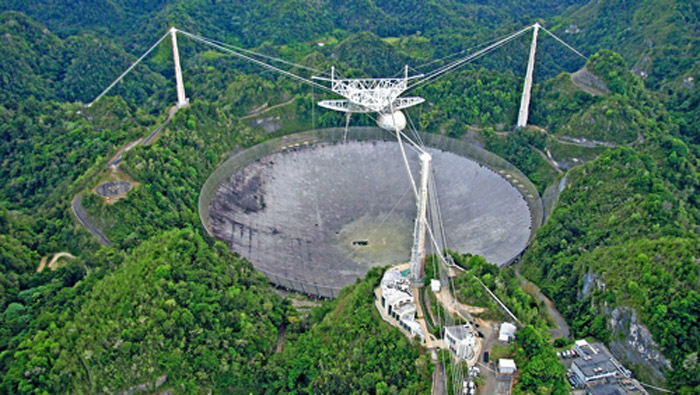
\includegraphics{images/20151101114231-0_8e7cc_c7a44aca_orig.jpg}}
\caption{\label{fig.arecibo} Arecibo telescope, in Puerto Rico.}
\end{subfigure}
\hfill
\begin{subfigure}{.43\textwidth}
\resizebox{\hsize}{!}{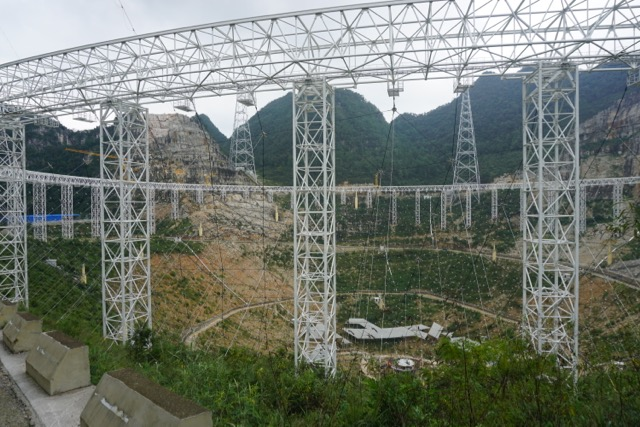
\includegraphics{images/FastTelescope_8sep2015.jpg}}
\caption{\label{fig.FAST} FAST telescope, in China}
\end{subfigure}
\caption{\label{fig.singleDishes} Examples of large single-dish radio telescopes.}
\end{figure}

\pg
Calibrating these dishes is a relatively straightforward matter - the signal loss and distortion as the dish converts the electromagnetic wave to a voltage can be described, based on the dish, either as a simple scaling factor, or a complex number (giving information on phase and amplitude errors). This loss and distortion model is referred to as the \emph{antenna gain}. Solving for these using more complex interferometric array is a problem described in Section \ref{section.calibration}.

\pg
For the remainder of this section, we will assume that calibration has been performed perfectly, and that the gain-corrections have been applied to voltage measurements. 

\section{Interferometry: Bypassing the Diffraction Limit}

\pg
There are two quantities of interest to astronomers of all stripes: sensitivity and resolution. An instrument's sensitivity is a function of its collecting area\footnote{It is also a function of technological factors, of course, but \emph{ceteris paribus}, a more sensitive telescope means a telescope with a wider collecting area}. Resolution, for well-designed instruments\footnote{By this, we mean that we assume that an instrument strives to optimise resolution.}, is limited by diffraction. This introduces issues specific to the radio domain. Radio waves, however, have very long wavelengths - often comparable to meters, rather than the 100$nm$ wavelengths of optical light. This introduces specific issues for astronomers, since achieving a resolution comparable to those of optical telescopes would require making telescopes with apertures tens of millions of times larger than those already titanic instruments!

\pg
To produce high-resolution maps of the radio sky, this technical limitation demands a technical solution. In practice, this solution consists of recourse to interferometric techniques. Indeed, interferometry can be thought of as the construction of a "sparse" dish, as illustrated in Fig.

\begin{figure}[h]
\centering
\begin{subfigure}{.43\textwidth}
\resizebox{\hsize}{!}{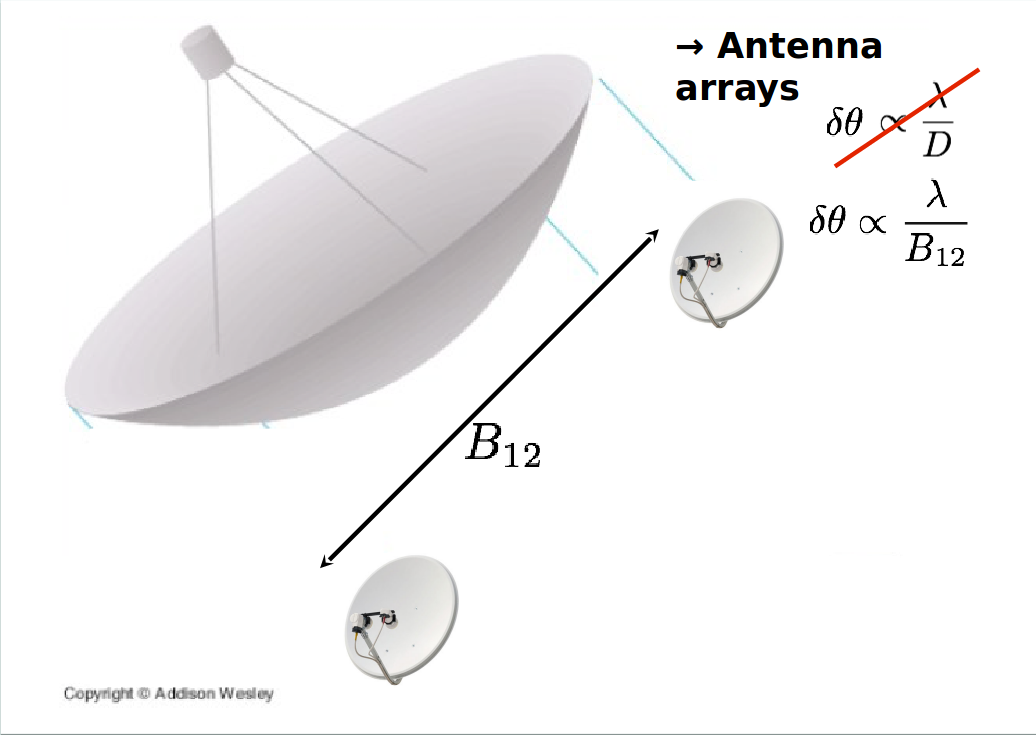
\includegraphics{images/baseline-resolution.png}}
\caption{\label{fig.baseline.image} A pair of dishes can surpass the resolution limit of its components.}
\end{subfigure}
\hfill
\begin{subfigure}{.43\textwidth}
\resizebox{\hsize}{!}{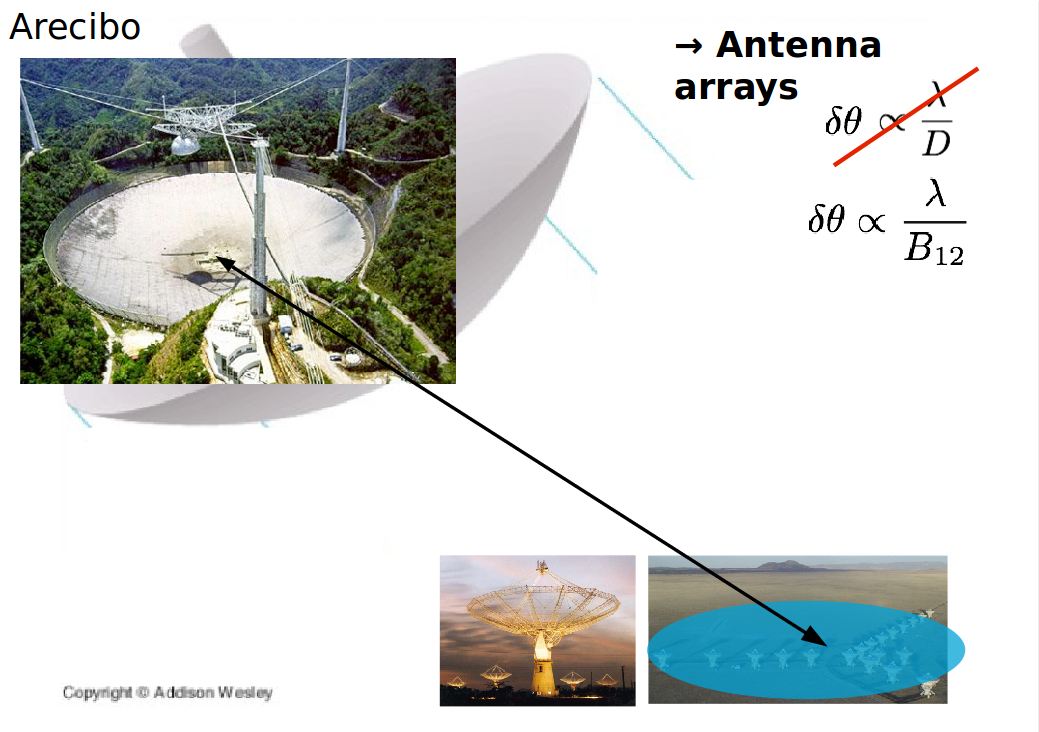
\includegraphics{images/arecibo-vla.png}}
\caption{\label{fig.arecibo.vla} With enough pairs of dishes, it is possible to synthesise a much larger dish.}
\end{subfigure}
\caption{\label{fig.aperture.synthesis} Illustration of the underlying principle of interferometry. The 27 dishes of the VLA can be thought of as "synthesising" a similar circular dish as Arecibo. This idea is the reason why radio interferometry is historically known as "aperture synthesis" in the literature of radio astronomy. Both images are copyrighted by Addison Wesley.}
\end{figure}

\pg
Of course, this improvement of resolution does not come for free. To understand the cost of interferometry, let us discuss the properties of its core component: the baseline.

\subsection{The Baseline}

\pg
To define the baseline, we must begin by considering the geometric properties of an interferometric array. For now, let us assume that we are observing the sky above the array, a practice known as drift-scanning. A baseline then consists of the vector subtraction of the positions, in 3-dimensional space, of its two constituent antennas. Note that each antenna pair therefore has 2 corresponding baselines, since for each pair of antennas A and B we have baselines AB and BA. These distance vectors are then divided by the observing wavelength to give a dimensionless set of coordinates, known as $(u,v,w)$. These coordinates define the baseline entirely. 

\subsection{The Visibility}

\pg
We have defined what a baseline corresponds to: a vector coordinate in $(u,v,w)$-space. To each baseline we associate a measurement, which we call the \emph{visibility}. 
\begin{figure}[h]
\centering
\resizebox{\hsize}{!}{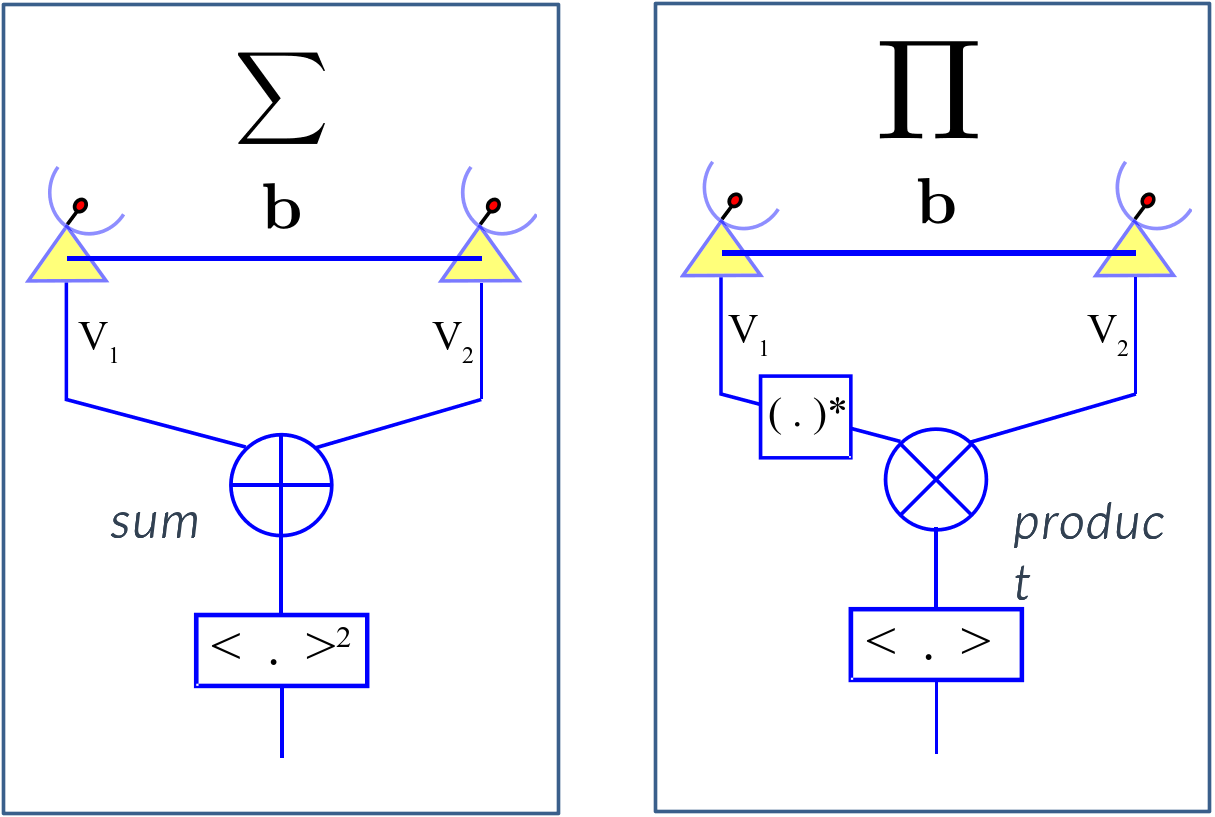
\includegraphics{images/visibility-creation.png}}
\caption{\label{fig.visibility} There are two ways to combine the voltages from two antennas into a visibility: they are sum-correlation and $\pi$-correlation. In this manuscript, we will only concern ourselves with the latter. Image credit: Julien Girard}
\end{figure}
The visibility associated with baseline $\mathbf{b}_{AB}$ is created by taking the voltage measured by antenna A, multiply it by the complex conjugate of the voltage measured by antenna B, average over the correlator dump time (i.e. the time over which the measurement is made). This scalar quantity is then multiplied by the baseline position vector. In other words:
\begin{equation}
\mathbf{b}_{AB} = V_{A} V_{B}^* \frac{\mathbf{x}_{B}-\mathbf{x}_{A}}{\nu_\mathrm{obs}}
\end{equation}

\pg
So we see that a visibility is a complex vector quantity. We also see that $\mathbf{b}_{AB} = \mathbf{b}_{BA}^*$: the information of the visibility associated with baseline BA is contained in the visibility associated with baseline AB. This means that in practice, only half of the visibilities ever need be stored. What does the visibility measurement correspond to?
\begin{figure}[h]
\centering
\resizebox{\hsize}{!}{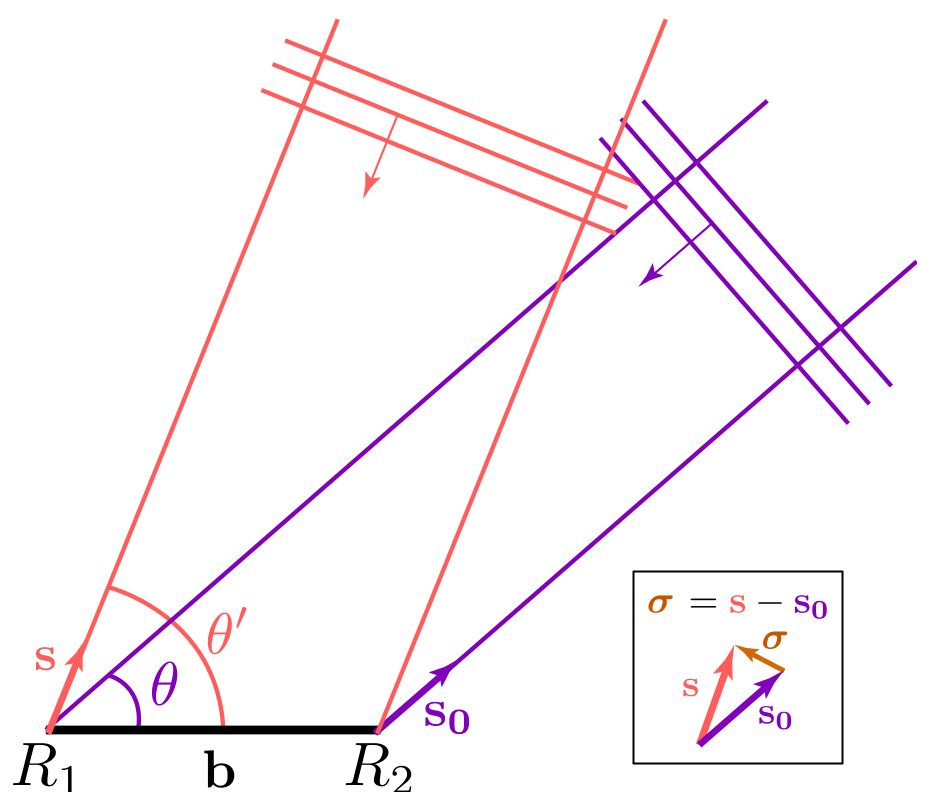
\includegraphics{images/visibility-measure.png}}
\caption{\label{fig.visibility.measure} Here, we assume that there are only two sources in the sky whose signal can be measured by our antennas. The final visibility is the sum of the visibilities associated with each individual source. Image credit: Julien Girard}
\end{figure}

\pg
The signals from various sources are additive in both antennas. Provided that the signal from both sources is coherent when observed by the dishes, the correlation between the total voltages will simply be the sum of the voltage correlations associated with individual sources - i.e. the interferometric signal from different sources are additive.

\pg
Note that in Fig. \ref{fig.visibility.measure}, neither source is at the zenith. We thus see that the \emph{effective baseline} which sees each source is in fact shorter than the \emph{physical baseline}. This can be corrected by digitally adding a phase delay in each antenna (or, in older interferometers, by playing with the cable length between each dish and the correlator) - this is in fact how interferometric arrays are pointed.

\subsection{The $uv$-plane}

\pg
In general, interferometric design is such that the $w$ component of visibilities' $(u,v,w)$ coordinates is negligible (or can be put in a frame of reference where it can usually be approximated as such). Radio astronomers tend to thus talk of a $uv$-plane rather than $uvw$-space to describe the space where visibilities live. The set of $uv$-values for all the baselines of an interferometric array is known as its $uv$-coverage, and defines the array's properties entirely.

\pg
For the VLA, for example, the $uv$-coverage when observing the zenith will be as shown in Fig. \ref{fig.vla.uvcoverage}.

\begin{figure}[h]
\centering
\resizebox{\hsize}{!}{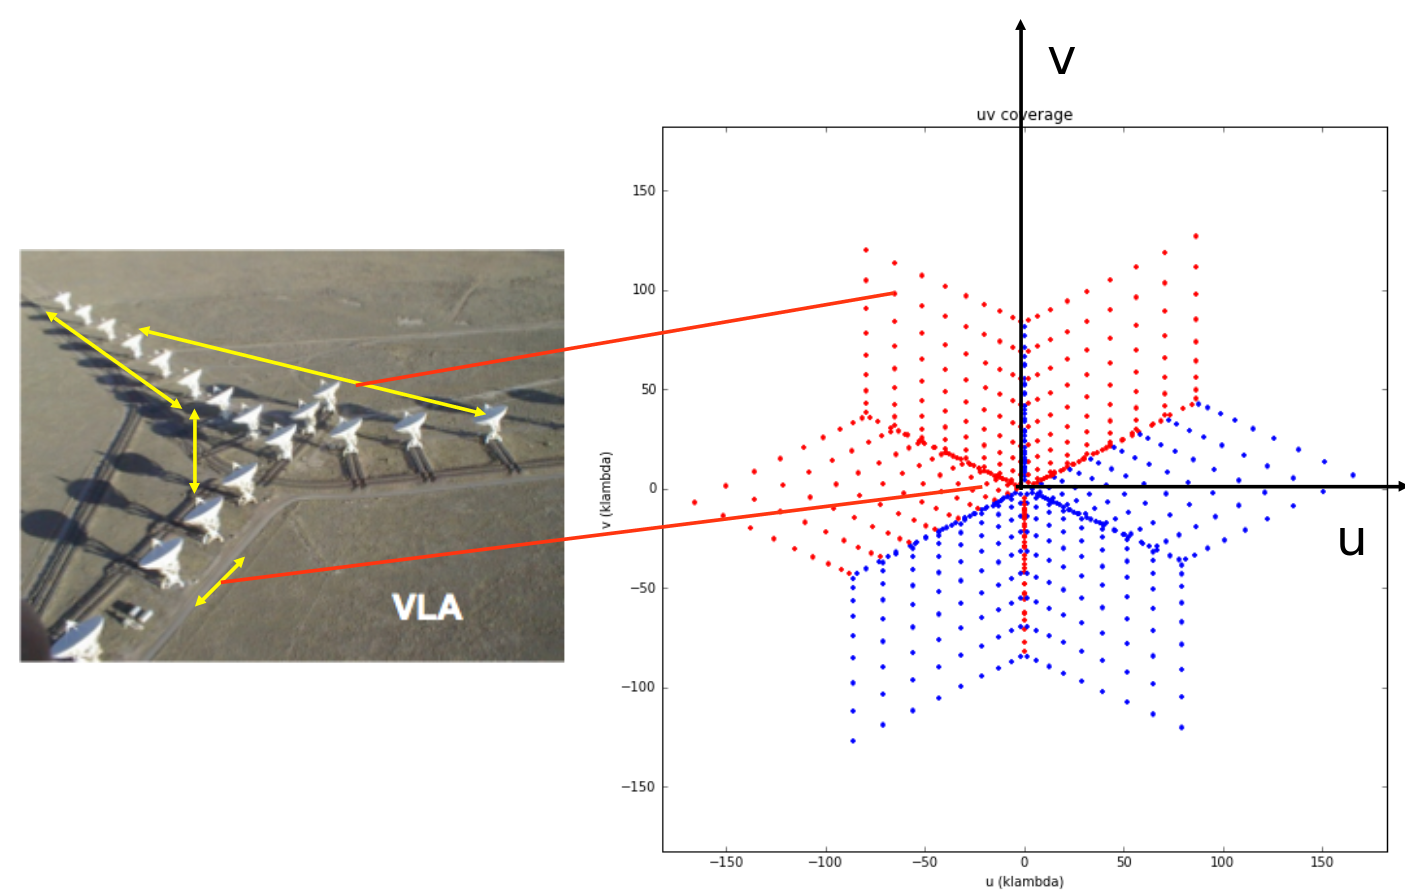
\includegraphics{images/vla-uvcoverage.png}}
\caption{\label{fig.vla.uvcoverage} The VLA contains 27 radio dishes placed as shown above. Each antenna pair between those 27 gives two single baselines, here, one red and one blue. Image credit: Julien Girard}
\end{figure}

%\pg
%The more points an array has in $uv$-space, the greater its $uv$-coverage and the better it will observe. This coverage can be improved for free in two main ways: firstly, the use of a technique known as supersynthesis (since the interferometer "synthesises" a dish at any given time, by assuming that the sky does not evolve over a certain time frame, we can treat different times as measurements of the same sky) and taking advantage of the frequency-dependence of $uv$-coordinates.The impact of both practices will be described in greater detail in \ref{sec.imag.psf}, but know that "$uv$-tracks" simply correspond to the $uv$-coverage of an interferometer observing over some period of time.

\pg
Individual antennas of an array can be pointed mechanically, and so the impact of pointing the interferometric array in a given direction can be minimised. But what happens to the array itself? It is useful here to go back to the illustration of Fig. \ref{fig.arecibo.vla}. Think of each dish in the array representing a "filled" segment of a massive but empty dish. By projecting our observation in a given direction, this dish goes from circular to elliptical.
\begin{figure}[h]
\centering
\begin{subfigure}{.40\textwidth}
\resizebox{\hsize}{!}{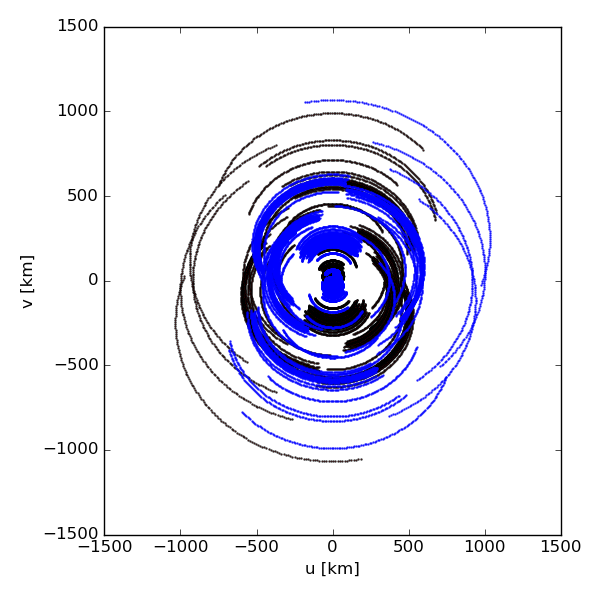
\includegraphics{images/lofar-uvcoverage-zenith.png}}
\caption{\label{fig.lofar.uvcoverage.zenith} $uv$-coverage of an 8-hour LOFAR observation when pointing at zenith..}
\end{subfigure}
\hfill
\begin{subfigure}{.40\textwidth}
\resizebox{\hsize}{!}{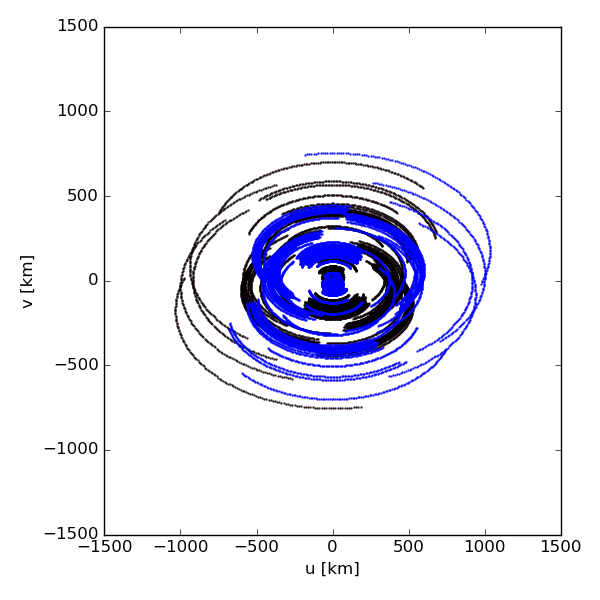
\includegraphics{images/lofar-uvcoverage-elsewhere.png}}
\caption{\label{fig.lofar.uvcoverage.elsewhere} $uv$-coverage of an 8-hour LOFAR observation when pointing 45 degrees away from zenith.}
\end{subfigure}
\caption{\label{fig.uvcoverage.lofar} Effect of array pointing on $uv$-coverage. By pointing the array 45 degrees in the $v$-axis, the array's $uv$-coverage (and thus maximum resolution) is decreased along the $v$-axis.}
\end{figure}


\subsection{The Point-Spread Function}\label{sec.imag.psf}

\pg
So far, we have seen that the purpose an interferometric array is to overcome the diffraction limit of single-dish antennas. We have described visibilities, which are the quantities measured by an interferometric array. What remains is to describe how these measurements are used to go make images of the sky.

\pg
Assuming that all the antennas in an array are equivalent and perfectly calibrated, the van Cittert-Zernike theorem (\citepads{1934Phy.....1..201V}, covered in \citepads{2001isra.book.....T}) allows us to equate a visibility with a single Fourier mode of the plane tangent to the sky where the instrument is pointed. This direction is called the \emph{phase centre}, because digital phase shifts are introduced between antenna voltages before averaging so as to point each visibility in this direction. 

\subsection{From Dirty to Clean: Mitigating the PSF}

\clearpage
% !TeX spellcheck = en_UK

\section{Calibration Methods in Radio Interferometry}\label{section.calibration}
\pg
In this section, we will discuss the implementation of interferometric array calibration. Our analysis is based on the RIME formalism, described in \cref{section.RIME}. One key metric of calibration quality is the \emph{dynamic range} (DR). High dynamic ranges mean that a high contrast has been obtained, and fainter sources can be reached. Dynamic range is defined as the following:
\begin{equation}\label{eq.DR}
DR = \frac{flux_{max}}{\max(\sigma_{thermal},\sigma_{artefacts})}
\end{equation}
where $flux_{max}$ is the flux of the brightest source, $\sigma_{thermal}$ the thermal noise in the image, and $\sigma_{artefacts}$ the noise associated with calibration artefacts.

\pg
The distinction between these two noise sources is crucial; one can never go `below noise' for a given observation, no matter the quality of calibration. Astronomers typically observe for longer periods of time in order to reduce $\sigma_{thermal}$ in their images, but this will not reduce the artefacts caused by poor calibration solutions. However, uncorrected Direction-Dependent Effects will not go away on their own, no matter how long the integration time.

\pg
There are three `generations' of calibration methods, of increasing complexity. I shall describe them in terms of the RIME, showing how each generation increases in generality to account for more exotic effects. For the sake of clarity, I shall henceforth refer to them interchangeably as `nth-generation calibration' or `nGC' methods.

\subsection{Generational Analysis}

\subsubsection{First-Generation: Open-Loop Calibration}\label{section.calibration.1gc}

\pg
First-generation calibration methods (1GC methods) consist of open-loop calibration. This relies entirely on instrument stability, and thus imposes significant design constraints on radio telescopes. It consists of briefly observing a calibrator before and after each observation run to find a gain factor and offset error\footnote{For a concrete example, see \href{http://www.analog.com/en/analog-dialogue/articles/open-loop-calibration-techniques.html}{here}.}

\pg
Phase calibration in the 1GC era `proper' was not done, as engineers were capable of ensuring phase stability in contemporary interferometers. Phase was thus calculated relative to a fixed frame of reference, usually the central antenna of a 3-antenna array. 

\pg
In RIME terms, this consists of solving for a very basic form of $\Gjones_p$:
\begin{equation}
\Gjones_p = \begin{bmatrix} a_p t + b_p \end{bmatrix} % \begin{bmatrix} e^{2 \pi i \nu ( \phi_p - \phi_0)} \end{bmatrix}
\end{equation}
where $a_p,b_p$ are constants solved for during open-loop calibration and $t$ is time. %, $\nu$ the observing frequency, $\phi$ the phase at an antenna, and $\phi_0$ the phase at the reference antenna.

\pg
While values for $a_p$ and $b_p$ can in theory be found for both autocorrelation and both crosscorrelations, low signal-to-noise means that in practice, a single set of values is solved for per antenna\footnote{This reduces calibration to solving only for the intensity gains: the data can then only be used for \emph{intensity mapping} (e.g. \citepads{1957IAUS....4..159J}). This practice therefore precludes polarimetry.}. With these techniques, one can achieve dynamic ranges of about 100:1 (\citepads{2010A&A...524A..61N}).

\subsubsection{Second-Generation: Self-Calibration}\label{section.calibration.2gc}

\pg
Second-generation calibration methods (2GC methods) are defined by their use of \emph{self-calibration}\footnote{On the discovery of self-calibration and its evolution in parallel to adaptive optics, I highly recommend the chapter titled "The Almost Serendipitous Discovery of Self-Calibration'' in "\href{http://library.nrao.edu/public/collection/02000000000280.pdf}{\citep{serendipitous}}.}, commonly referred to as \emph{self-cal} (\citepads{1984ARA&A..22...97P}). As described in \cref{section.RIME.FullSky.CVZ}, this method can only be deployed if the brightness matrix of the sky is the same for all baselines\footnote{This is not to say that the brightness matrix must contain only point sources, but rather that moving our interferometer 500m to the East should not change its measured visibilities} (i.e. that we are not affected by direction-dependent effects).

\pg
The seeds of self-calibration (and adaptive optics) is a paper published in the era of 1GC by Jennison (\citepads{1958MNRAS.118..276J}, expanding on his PhD work, which was published in 1951). With sufficient signal-to-noise, he showed that \emph{phase closure} could be calculated and errors due to the atmosphere thus mitigated.

\pg
Self-calibration and adaptive optics are the same thing, albeit meeting different constraints. Most notably, interferometric data is digital, allowing radio astronomers to perform their adaptive optics correction after the observation.

\pg
[ TODO: put adaptive optics diagram here maybe]

\pg
If amplitude and phase gains can be written as antenna-dependent, then each antenna-based error is estimated N times (once per baseline which includes this antenna). By estimating, and correcting for, these errors, one can use a simple source model to infer an improved one. This is why the method is referred to as self-cal; by calibrating `on' a good calibrator source (bright, compact and unresolved), one can drastically improve one's source model, along with one's calibration solutions.

\pg
By extending this idea to VLBI\footnote{e.g.  \citepads{1974ApJ...193..293R}}, \emph{amplitude closure} was introduced to the field along with phase closure \citepads[as described in][]{1983Sci...219...51R}. Astronomers were quick to apply these methods to interferometers in general.

\pg
The great advantage of radio interferometry over optics, however, is that we can \emph{iterate} over progressively improved source models. This is because interferometric data is digital, and because we record phase information.

\pg
In practice, of course, self-cal will be limited by noise. More precisely, it will be limited by sensitivity, in the form of the signal-to-noise ratio (henceforth SNR). For sufficiently bright sources, with high SNR, self-calibration can easily improve dynamic range by a factor of 10 (\cite{serendipitous}, p. 154) in a single iteration. 

\subsubsection{Third-Generation: Direction-Dependent Effects}

\pg
Third-generation calibration (3GC) is an extension of 2GC calibration which takes direction-dependent effects into account. At the time of writing, this is the cutting edge in radio interferometric calibration.

\pg
In this section, I will discuss the approach taken by [cite DDF and kMS paper when it comes out] and [cite prefactor paper if/when it is out], \emph{facet-based calibration}. This method has an imaging equivalent \citepads[see][and associated papers]{2017arXiv171202078T}. The approach cannot be divorced from imaging, for the simple reason that solving for and applying Jones matrices in different directions requires image-plane knowledge of the sky brightness distribution $\Bmatrix$. The imaging challenges this methods introduces will be discussed in [href to relevant imaging section].

\pg
The crucial insight of this approach consists 







\clearpage

\section{The Low-$\nu$ Sky: Emission Mechanisms}
\pg
This section aims to bring a brief introduction to the emission mechanisms which dominate at low frequencies, and thus determine the physics accessible to extragalactic astronomers working in this band. Specifically, it will briefly describe thermal radiation detected at low frequencies (associated with dust \& protoplanetary disks, and therefore a tracer of star formation) along with free-free radiation (which is emitted from ionised plasma outflows, and thus a tracer of various physical objects e.g. young stellar objects - cf. \citet{2017ApJ...834..206C} - and starburst regions - cf. \citet{2015A&A...574A.114V}) and synchrotron radiation, which is a tracer of more violent and energetic processes (and thus associated with supernova remnants, AGN, or radio halos - cf. \citet{2010A&A...509A..68C}).

\pg
Of course, each individual galaxy will have differing contributions from different mechanisms - in practice, when studying galactic populations, the overall flux at a given frequency will simply be summed up for each galaxy and become one point in a Spectral Energy Distribution, or SED. However, when studying individual objects, it can be critical to understand which emission mechanism dominates at what frequencies. %: it will be very difficult to find traces of star formation in the emission from a galaxy dominated by an AGN, for example. Along with a brief introduction of the main emission mechanisms, then, we will give the characteristic spectrum of each, to show how different types of emission can be differentiated in practice.
For example, the radio and far-infrared spectrum for nearby M82 are shown in Fig. \ref{plot.m82.spectrum}\footnote{Figure and work taken from the NRAO website. For further information, \href{https://www.cv.nrao.edu/course/astr534/FreeFreeEmission.html}{see here}}.
\begin{figure*}[!h]
\centering
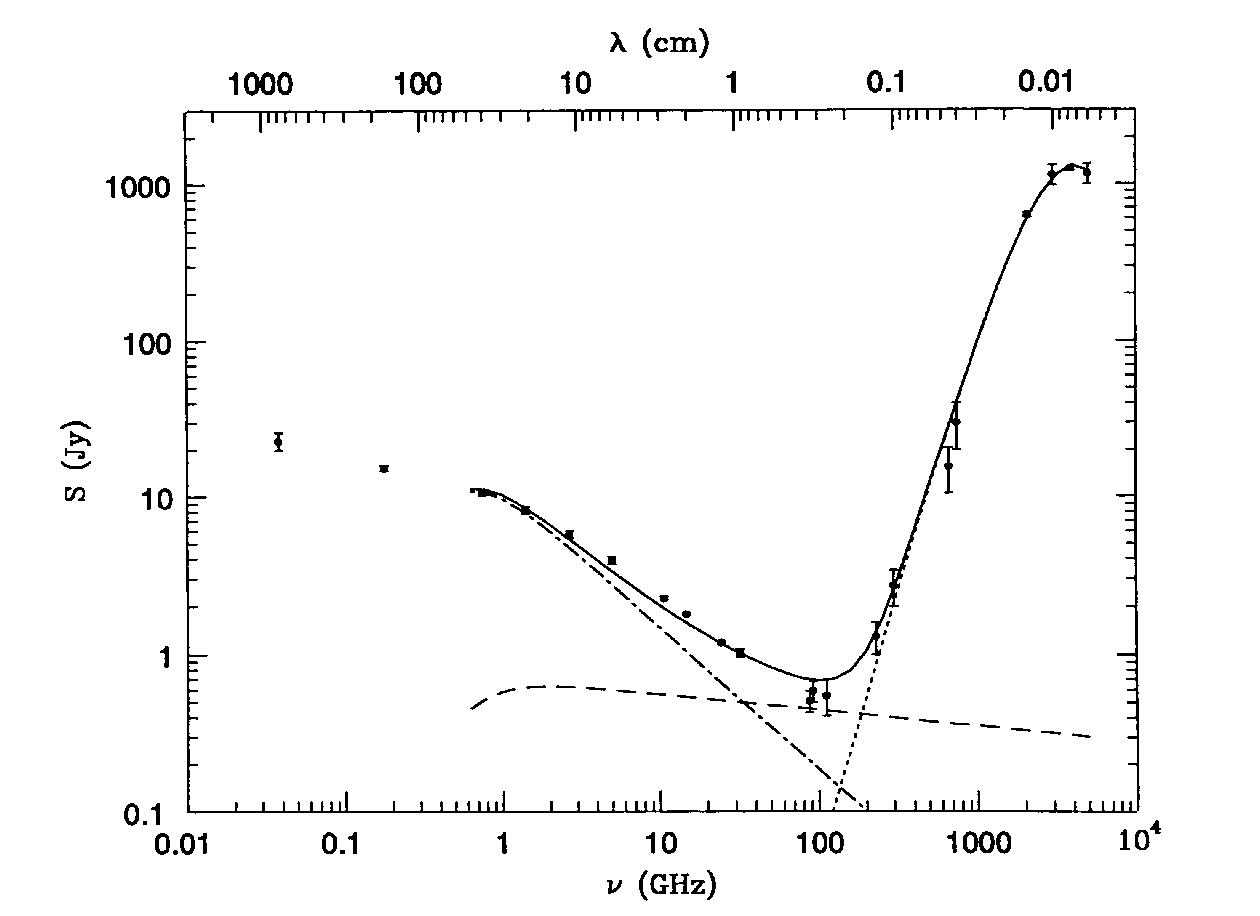
\includegraphics[width=\textwidth]{images/M82Spectrum.png}
\caption{\label{plot.m82.spectrum} Radio and far-infrared spectrum for galaxy M82, as estimated \href{https://www.cv.nrao.edu/course/astr534/FreeFreeEmission.html}{by the NRAO online course}. The flat curve corresponds to free-free emission, while synchrotron radiation and thermal dust emission dominate at low and high frequencies respectively.}
\end{figure*}

\pg


\subsection{Thermal Radiation}
\pg
Also known as black-body radiation, its spectral intensity is given by Planck's law, given in Eq. \ref{eq.planck}.
\begin{equation}\label{eq.planck}
%B_\lambda (\lambda,T) = \frac{2hc^2}{\lambda^5}\left(e^{\frac{hc}{\lambda k_BT}}-1\right)^{-1}
B_\nu(\nu,T) = \frac{2h\nu^3}{c^2}\left(e^\frac{h\nu}{k_BT}-1\right)^{-1}
\end{equation}
where $B_\lambda$ is the flux density at frequency $\nu$ for a source with temperature $T$, and $k_B=1.381 \left[J/K\right]$ is the Boltzmann constant. Near protostellar disks, synchrotron emission is absorbed by the ambient interstellar medium, heating it up to an average of $\sim 10^4$ (see \citetads{2009ApJS..181..255A}, \citetads{1978ppim.book.....S} and references therein). This gives the following spectral curve:

\begin{figure*}[!h]
\centering
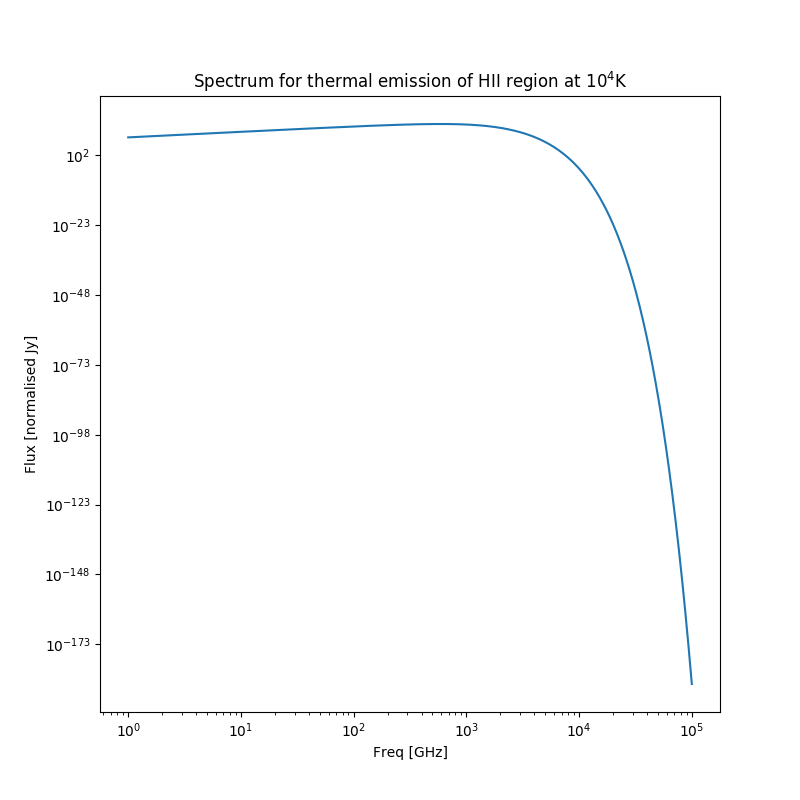
\includegraphics[width=0.8\textwidth]{images/ThermalEmission.png}
\caption{\label{plot.thermal}Log-Log plot of blackbody radiation emitted by a particle at $10^4$ Kelvin. Note that the y-axis is arbitrary, since it will in practice be modulated by the number of particles in a region, radiation efficiency, resolution etc.}
\end{figure*}
\pg
This is the dominant mode of emission for distant galaxies in the infrared band. In the LOFAR regime, it is not expected to dominate for extragalactic sources, but ought to be detected for resolved galaxies.

\subsection{Free-Free Radiation}
\pg
Free-free or ``bremsstrahlung" (``braking") radiation occurs when the trajectory of a high-energy charged particle is deflected by an electric field. This non-thermal emission mechanism is the dominant mechanism in HII regions (which contain ionised hydrogen), where star formation has previously taken place. It is called free-free emission because it is produced by free electrons scattering off ionised hydrogen without being captured. % as shown in Fig. \ref{plot.freefree}
%\begin{figure*}[!h]
%\centering
%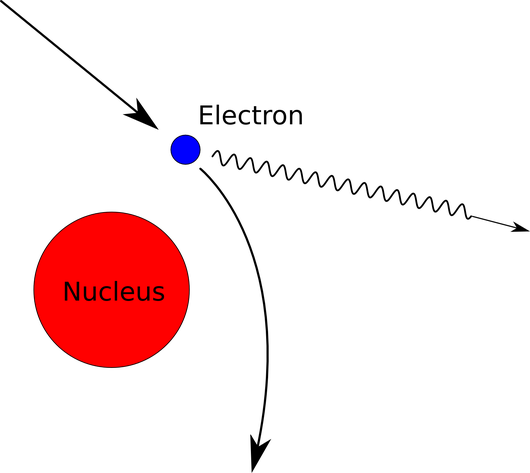
\includegraphics[width=0.3\textwidth]{images/bremsstrahlung.png}
%\caption{\label{plot.freefree} Schematic showing the physical process leading to free-free emission. As we can see, the electron is scattered, but not captured. Source: \url{https://thephysicsbehind.com/2015/04/16/x-ray-tubes/}}
%\end{figure*}

\pg
This emission's spectrum is heavily dependent on a number of factors: including frequency, temperature, and critically, free-free opacity $\tau_\nu$, itself a function of electron density. It is characterised by a knee in its spectrum, occurring where $\tau_\nu\sim 1$. This knee delineates two regions with different spectral indices; $\alpha \sim -0.1$ at higher frequencies, and $\alpha \leq 2$ at lower frequencies. This gives a characteristic shape, shown in Fig. \ref{plot.freefree.spectrum}.
\begin{figure*}[!h]
\centering
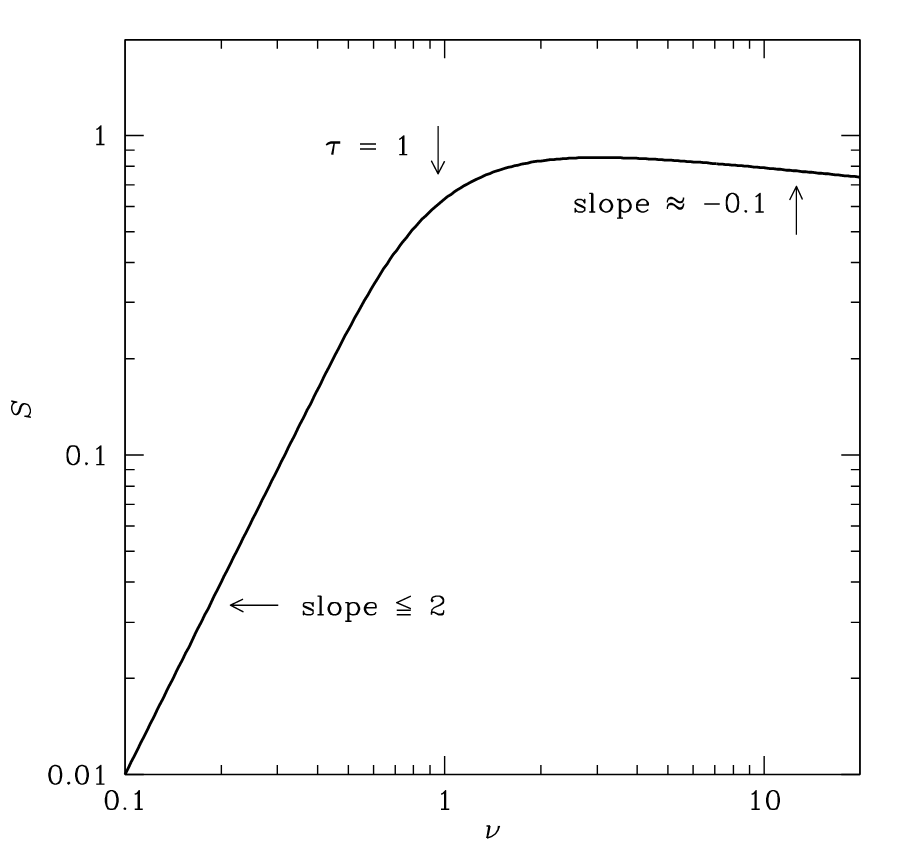
\includegraphics[width=0.9\textwidth]{images/freefree.png}
\caption{\label{plot.freefree.spectrum} Characteristic spectrum of free-free radiation. Arbitrary unit scale. Source: NRAO online course.}
\end{figure*}

\pg
As we can see, this spectrum falls off sharply with frequency. As such, while it is expected to dominate over thermal emission in the absence of synchrotron radiation, it is unlikely to dominate in the LOFAR band. It acts as a tracer for star formation and other "gentler" physical processes detected at low radio frequencies.

\subsection{Synchrotron Radiation}
\pg
Synchrotron radiation (or "magnetobremsstrahlung") occurs when the trajectory of a high-energy charged particle is deflected by a magnetic field. As the German name suggests, it is the magnetic equivalent of free-free radiation. It is the tracer of extremely violent processes, such as AGN jets. In its mildly relativistic regime, it is referred to as cyclotron radiation, after the device in which it was first tested, and in non-relativistic regimes, it is known as gyro radiation. 

\pg






\clearpage
\section{LOFAR: The LOw-Frequency Array}

\pg
In this section, we will describe the LOw Frequency Array LOFAR \citepads{2013A&A...556A...2V}, its technical properties and its current state of the art. In particular, the distinction between "Dutch" LOFAR and "international" LOFAR - and the technical problems associated with each - will be made explicit in this section.

\pg
LOFAR is a SKA pathfinder instrument, which means that it serves not only as a cutting-edge instrument in its own right, but does so with the explicit aim of serving as testing grounds for technologies \& techniques which could be usefully implemented in the SKA. It is in this context, for example, that trailblazers such as NeNuFar \citepads{2012sf2a.conf..687Z}, a low-frequency extension of LOFAR, are tested. LOFAR is an interferometric array, meaning that it consists of antennas which are combined to form stations, which are themselves distributed throughout the Netherlands and Europe.
\begin{figure}[h!] 
  \begin{minipage}[c]{0.45\linewidth}
    \centering
    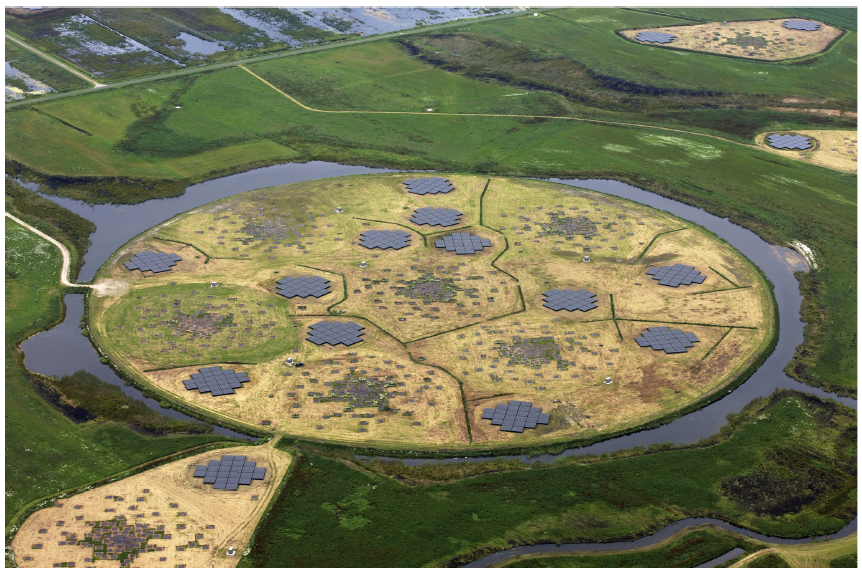
\includegraphics[width=\linewidth]{images/superterp.png}
	\subcaption{\label{fig.lofar.superterp} LOFAR core, known as the Superterp.}
%    \vspace{4ex}
  \end{minipage}
  \hfill
  \begin{minipage}[c]{0.45\linewidth}
    \centering
    \includegraphics[width=.5\linewidth]{images/{lofar-core-map_grey.jpg}}
    \subcaption{\label{fig.lofar.core} Distribution of the so-called LOFAR "core" stations, which include the Superterp.}
%    \vspace{4ex}
  \end{minipage} 
  \begin{minipage}[c]{0.45\linewidth}
    \centering
    \includegraphics[width=\linewidth]{images/{Distribution_Remote_Stations}} 
    \subcaption{\label{fig.lofar.remote} LOFAR with both "core" and "remote" stations.}
%    \vspace{4ex}
  \end{minipage}
  \begin{minipage}[c]{0.45\linewidth}
    \centering
    \includegraphics[width=.9\linewidth]{images/{Distribution_International_Stations}} 
    \subcaption{\label{fig.lofar.international} International LOFAR. Newer stations (one in Ireland, three in Poland) are not shown here.}
%    \vspace{4ex}
  \end{minipage} 
\caption{\label{fig.lofar.distribution} Geographic location and distribution of LOFAR stations, explicitly showing what is meant by Superterp, core, remote and international stations. All images from \href{https://www.astron.nl/radio-observatory/astronomers/users/technical-information/lofar-array-configuration/lofar-array-conf}{the official ASTRON website}}
\end{figure}


\pg
There are two bands to LOFAR, which are known as LOFAR-HBA (High-Band Antennas) and LOFAR LBA (Low-Band Antennas). \cref{fig.lofar.superterp,fig.fr606.layout} show the layout of the 6 innermost core stations and the French international LOFAR station, respectively.
\begin{figure}[h!]
\includegraphics[width=0.5\textwidth]{images/{LOFAR_NenuFAR.jpg}}
\caption{\label{fig.fr606.layout} Layout of FR606, the French LOFAR station at Nancay. At bottom left are the HBA tiles, bottom right the LBA dipoles, and at the top are some of the NenuFAR mini-arrays.}
\end{figure}



\pg
We see the presence, in both cases, of two very different antenna types. One of these antenna types is not a single antenna, but rather a phased array: 16 antenna dipoles distributed in a $4 \times 4$ array. LOFAR stations include 48 such tiles, distributed in a cross pattern. This pattern is shown in \cref{fig.hba.tile}. Core stations HBA tiles are split into two 24-tile crosses. The antennas from each tile are combined into a phased array with a single ``tile beam", and all tile beams are themselves combined into a station beam\footnote{Referece: \href{https://www.astron.nl/radio-observatory/astronomers/technical-information/antennae/antennae-description}{ASTRON technical description}}. This station beam is then pointed digitally.
\begin{figure}[h!]
\includegraphics[width=0.45\textwidth]{images/{Schematic-diagram-of-a-24-tile-LOFAR-HBA-station-A-tile-is-made-of-16-dual-polarization.png}}
\caption{\label{fig.hba.tile} Layout of a single HBA tile. Source: \href{https://www.researchgate.net/profile/Sarod_Yatawatta/publication/281316394/figure/fig1/AS:614002589720576@1523401033149/Schematic-diagram-of-a-24-tile-LOFAR-HBA-station-A-tile-is-made-of-16-dual-polarization.png}{Sarod Yatawatta researchgate profile}}
\end{figure}

\pg
LOFAR-HBA is sensitive to higher frequencies, from 120 MHz to 240 MHz\footnote{Reference: \href{http://www.lofar.org/about-lofar/system/lofar-numbers/lofar-numbers}{LOFAR.org website}}. It has a smaller field of view than LOFAR-LBA, but a better resolution. 

\pg
LBA antennas, meanwhile, follow a very simple - and cost-effective - design. A typical LBA antenna is shown in \cref{fig.lba.ant}. 96 such antennas are spread in a semi-random pattern in each LOFAR station\footnote{Reference: \href{http://www.lofar.org/about-lofar/system/lofar-numbers/lofar-numbers}{LOFAR.org website.}}. In survey observations, they are combined as a single phased array.
\begin{figure}[h!]
\includegraphics[width=0.45\textwidth]{images/{lba.png}}
\caption{\label{fig.lba.ant} Picture of a single LBA antenna. Source: \href{https://i2.wp.com/lofar.ie/wp-content/uploads/2017/04/lba.png?resize=1500\%2C1000}{LOFAR technology website.}}
\end{figure}

\pg
The dipole design frees observers from the need to physically point antennas at all: the final station pointing is achieved by digitally introducing delays in observed phase before averaging the data. In this sense, the pointing is achieved in the same way as individual HBA tile pointing, but with one less degree of complexity. These antennas are receptive to signals emitted in the 30-80 MHz frequency range.

\pg
At the time of writing, use of the LBA data is still relatively new, as its calibration is a very tricky problem. For similar reasons, international LOFAR (i.e. the full LOFAR array) has not been used, at the time of writing, to create wide-field survey images. A large part of the work described in this manuscript consists of reaching a point where full use can be made of international LOFAR, in a streamlined and repeatable way. 



\chapter{Analysing the Variance of Gain Solutions}
put paper in there once it's refereed
%\input{source/EtiennePaper1/thesis-paper.tex}

%\input{source/intro.teximaging.tex}
%\newpage
%% !TeX spellcheck = en_UK

\section{Calibration Methods in Radio Interferometry}\label{section.calibration}
\pg
In this section, we will discuss the implementation of interferometric array calibration. Our analysis will be based on the RIME formalism described in \cref{section.RIME}. One key metric of calibration quality is the \emph{dynamic range} (DR). High dynamic ranges mean that a high contrast has been obtained, and fainter sources can be reached. Dynamic range is defined as the following:
\begin{equation}\label{eq.DR}
DR = \frac{flux_{max}}{\max(\sigma_{thermal},\sigma_{artefacts})}
\end{equation}
where $flux_{max}$ is the flux of the brightest source, $\sigma_{thermal}$ the thermal noise in the image, and $\sigma_{artefacts}$ the noise associated with calibration artefacts.

\pg
The distinction between these two noise sources is crucial; one can never go `below noise' for a given observation, no matter the quality of calibration. Astronomers typically observe for longer periods of time in order to reduce $\sigma_{thermal}$ in their images, but this will not reduce the artefacts caused by poor calibration solutions. However, uncorrected Direction-Dependent Effects will not go away on their own, no matter how long the integration time.

\pg
There are three `generations' of calibration methods, of increasing complexity. I shall describe them in terms of the RIME, showing how each generation increases in generality to account for more exotic effects. For the sake of clarity, I shall henceforth refer to them interchangeably as `nth-generation calibration' or `nGC' methods.

\subsection{First-Generation: Open-Loop Calibration}\label{section.calibration.1gc}

\pg
First-generation calibration methods (1GC methods) consist of open-loop calibration. This relies entirely on instrument stability, and thus imposes significant design constraints on radio telescopes. It consists of briefly observing a calibrator before and after each observation run to find a gain factor and offset error\footnote{For a concrete example, see \href{http://www.analog.com/en/analog-dialogue/articles/open-loop-calibration-techniques.html}{here}.}

\pg
Phase calibration in the 1GC era `proper' was not done, as engineers were capable of ensuring phase stability in contemporary interferometers. Phase was thus calculated relative to a fixed frame of reference, usually the central antenna of a 3-antenna array. 

\pg
In RIME terms, this consists of solving for a very basic form of $\Gjones_p$:
\begin{equation}
\Gjones_p = \begin{bmatrix} a_p t + b_p \end{bmatrix} % \begin{bmatrix} e^{2 \pi i \nu ( \phi_p - \phi_0)} \end{bmatrix}
\end{equation}
where $a_p,b_p$ are constants solved for during open-loop calibration and $t$ is time. %, $\nu$ the observing frequency, $\phi$ the phase at an antenna, and $\phi_0$ the phase at the reference antenna.

\pg
While values for $a_p$ and $b_p$ can in theory be found for both autocorrelation and both crosscorrelations, low signal-to-noise means that in practice, a single set of values is solved for per antenna\footnote{This reduces calibration to solving only for the intensity gains: the data can then only be used for \emph{intensity mapping} (e.g. \citepads{1957IAUS....4..159J}). This practice therefore precludes polarimetry.}. With these techniques, one can achieve dynamic ranges of about 100:1 (\citepads{2010A&A...524A..61N}).

\subsection{Second-Generation: Self-Calibration}\label{section.calibration.2gc}

\pg
Second-generation calibration methods (2GC methods) are defined by their use of \emph{self-calibration}\footnote{On the discovery of self-calibration and its evolution in parallel to adaptive optics, I highly recommend the chapter titled "The Almost Serendipitous Discovery of Self-Calibration'' in "\href{http://library.nrao.edu/public/collection/02000000000280.pdf}{\citep{serendipitous}}.}, commonly referred to as \emph{self-cal} (\citepads{1984ARA&A..22...97P}). As described in \cref{section.RIME.FullSky.CVZ}, this method can only be deployed if the brightness matrix of the sky is the same for all baselines\footnote{This is not to say that the brightness matrix must contain only point sources, but rather that moving our interferometer 500m to the East should not change its measured visibilities} (i.e. that we are not affected by direction-dependent effects).

\pg
The seeds of self-calibration (and adaptive optics) is a paper published in the era of 1GC by Jennison (\citepads{1958MNRAS.118..276J}, expanding on his PhD work, which was published in 1951). With sufficient signal-to-noise, he showed that \emph{phase closure} could be calculated and errors due to the atmosphere thus mitigated.

\pg
Self-calibration and adaptive optics are the same thing, albeit meeting different constraints. Most notably, interferometric data is digital, allowing radio astronomers to perform their adaptive optics correction after the observation.

\pg
[ TODO: put adaptive optics diagram here maybe]

\pg
If amplitude and phase gains can be written as antenna-dependent, then each antenna-based error is estimated N times (once per baseline which includes this antenna). By estimating, and correcting for, these errors, one can use a simple source model to infer an improved one. This is why the method is referred to as self-cal; by calibrating `on' a good calibrator source (bright, compact and unresolved), one can drastically improve one's source model, along with one's calibration solutions.

\pg
By extending this idea to VLBI\footnote{e.g.  \citepads{1974ApJ...193..293R}}, \emph{amplitude closure} was introduced to the field along with phase closure, as described in \citepads{1983Sci...219...51R}. Astronomers were quick to apply these methods to interferometers in general.

\pg
The great advantage of radio interferometry over optics, however, is that we can \emph{iterate} over progressively improved source models. This is because interferometric data is digital, and because we record phase information.

\pg
In practice, of course, self-cal will be limited by noise. More precisely, it will be limited by sensitivity, in the form of the signal-to-noise ratio (henceforth SNR). For sufficiently bright sources, with high SNR, self-calibration can easily improve dynamic range by a factor of 10 (\cite{serendipitous}, p. 154) in a single iteration. 

\subsection{Third-Generation: Direction-Dependent Effects}

\pg
Third-generation calibration (3GC) is an extension of 2GC calibration which takes direction-dependent effects into account. At the time of writing, this is the state of the art in radio interferometric calibration.

\pg
In this section, I will discuss the approach taken by [cite DDF and kMS paper when it comes out] and [cite prefactor paper if/when it is out], \emph{facet-based calibration}. The approach cannot be divorced from imaging, for the simple reason that solving for and applying Jones matrices in different directions requires image-plane knowledge of the sky brightness distribution $\Bmatrix$. The imaging challenges this methods introduces will be discussed in [href to relevant imaging section].

\pg








%\newpage

%\chapter{Observational Work}

\chapter{Scientific Strategy}

\section{3C295 and the Extended Groth Strip}

\pg
Observe \& Model 3C295 to get amplitude calibration over entire LOFAR bandwidth


\section{Imaging the Full Primary Beam}
\pg
Perform DID calibration at low resolutions (no international baselines) to get complete, approximatemodel of entire EGS field

\section{Test Decorrelation}
\pg
see effect of decorrelation on LOBOS sources around EGS as function of distance from 3c295 - talk about two sources of decorrelation (direction-dependent PSF, which is modelled, and gains changing with direction, which is unmodelled and will have an impact in image). See maximum impact of gain-decorrelation: we want flat decorrelation as function of distance from 3c295.

\section{Imaging the EGS with LOFAR international stations}
\pg
if decorrelation is merciful, proceed to patchwise imaging of EGS by using the results from the sections above (DI calibration using 3c295 model, followed by subtraction of all sources seen at low-res except within the patch we want to image; image, change patch; repeat until all EGS imaged)

\newpage

\chapter{Imaging 3C295 with International LOFAR}\label{section.3c295}
\minitoc
% % % % % % % % % % % % % % % % % % % % % % %
\section{Aims \& Methodology}
\pg
Our aim in this section is to create a high-resolution model of 3C295, something that - as
of yet - does not exist. More specifically, we seek to create a model that will allow us to find
good phase-calibration solutions for LOFAR international baselines. While we also solve for
amplitude gains, we know that we will need to correct the total source flux in each frequency
subband as our initial spectral model is not necessarily correct.
We select 6 sub-bands out of the total LOFAR HBA bandwidth, evenly spread throughout the bandwidth as shown in Fig. \ref{fig.freqsamp}.

\pg
This approach should allow us to appropriately constrain the final spectral behaviour of our high-resolution model, once the amplitude correction is applied to ensure our model is compliant with pre-existing flux measurements for this source \citepads{arse}. [put image of source flux as function of frequency for 3c295, citing source and ideally showing position of our subbands]

\pg
Our procedure is as follows: we self-calibrate individual subbands, starting from a model
extracted from a high-resolution VLA observation of 3C295 at 8.7 GHz \citepads[cf.][]{1991AJ....101.1623P}. Once this is done,
we extract and apply a scalar flux correction factor for each subband so that the integrated flux of our 3C295 image is compatible with the existing literature at all frequencies. The resulting model is then reliable enough to calibrate our Groth Strip data using the full LOFAR array and the entire HBA bandwidth.

% % % % % % % % % % % % % % % % % % % % % % %
\section{Data Reduction}

\subsection{Data \& Observation Properties}
\pg
The dataset used for this PhD project is part of the LOFAR Surveys KSP Tier-1 survey, which consists of a number of 8-hour pointings covering as much of the sky visibile to LOFAR as possible. We analyse one of these pointings, an observation performed on the 28th of August 2014 and centred on the Extended Groth Strip. As part of the Tier-1 survey, it is an 8-hour-long observation. We limit ourselves to analysing only the HBA observation, meaning that we use 365 sub-bands which sample a total bandwidth of [give bandwidth]. We use all Core and Remote LOFAR stations, as well as some of the International stations which were online at the time (specifically the German stations 1-5 and 7, along with the Swedish and the British station).

\pg
The data was acquired through the LOFAR Long-Term Archive, and is thus pre-processed and flagged for RFI using the standard tools ([cite aoflagger, ndppp?]). 

\subsection{Calibrating the Data}
\pg
Since we plan on applying an amplitude correction based on the works of Scaife \& Heald \citep[see][]{arse}, our overriding concern is to find good phase and amplitude gain without concern for the overall scaling factor. As such, our calibration strategy consists of calibrating 6 subbands, chosen across the LOFAR bandwidth, simultaneously. The chosen subbands, and their position in the total bandwidth, are shown here:
\begin{figure}[h]
\begin{floatrow}
\ffigbox{%
  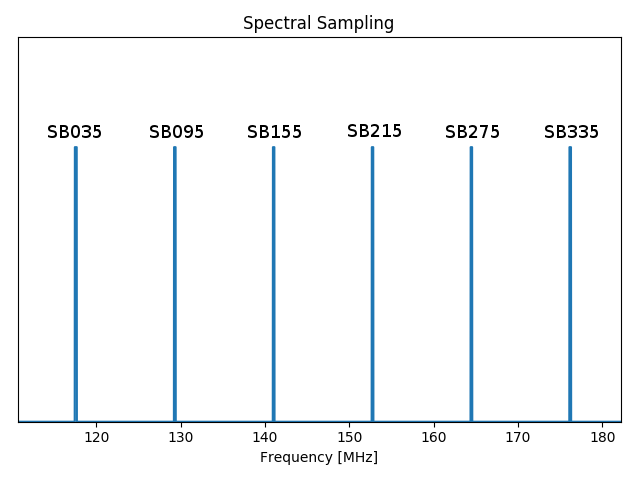
\includegraphics[width=0.5\textwidth]{images/FreqSampLabelled}
}{%
  \caption{\label{fig.freqsamp}Position of subbands chosen across full LOFAR bandwidth}%
}
\capbtabbox{%
  \begin{tabular}{|cc|} \hline
  Subband & $\nu_\mathrm{min} - \nu_\mathrm{max}$ \\ \hline
  SB035   &  117.45-117.69\\
  SB095   & 129.21-129.41\\
  SB155   & 140.93-141.12\\
  SB215   & 152.65-152.84\\
  SB275   & 164.37-164.56\\
  SB335   &  176.08-176.28 \\\hline
  \end{tabular}\vspace{1.2cm}
}{%
  \caption{Frequency bounds for the subbands chosen}%
}
\end{floatrow}
\end{figure}

\pg
Because no high-resolution models exist for 3C295 at our observing frequencies, which span quite a large bandwidth, care must be taken not to bias our model in an unphysical direction. We acquire the initial calibration model by extracting features from a NASA/IPAC Extragalactic Database\footnote{\hyperref[here]{https://ned.ipac.caltech.edu/}} image of 3C295 \citepads[see][]{1991AJ....101.1623P}, shown in Fig. \ref{fig.vla.3c295}. This feature extraction is carried out using PyBDSM \citepads{2015ascl.soft02007M}, changing all extracted Gaussians into points\footnote{This practice ensures that wrongly-estimated Gaussians do not end up introducing unphysical bias during calibration.}.
\begin{figure}[h]
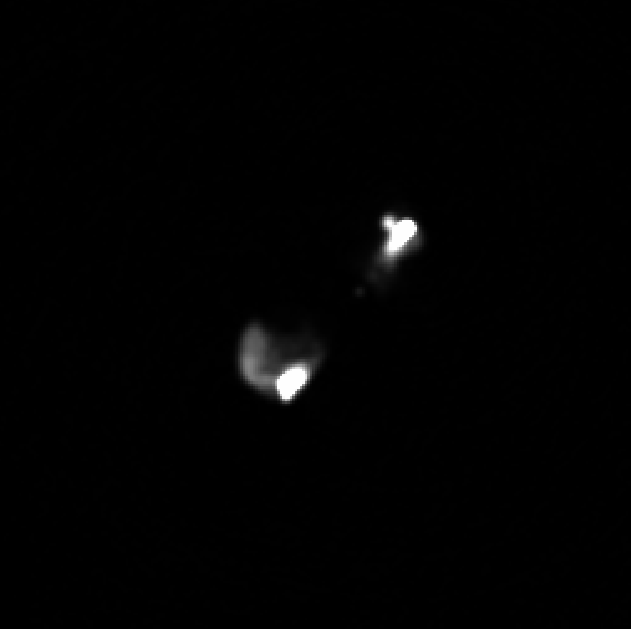
\includegraphics[width=0.4\linewidth]{images/3c295-vla}
\caption{\label{fig.vla.3c295}VLA observation of 3C295 at 8.7 GHz. Pixel size is $0.2''$.}
\end{figure}

\pg
For SB035, the gain curves for all antenna when calibrating with the initial model are as shown in Fig \ref{fig.sb035.gains.pass1}. Note that, especially for the international baselines, the gain amplitudes show a lot of structure: this is unphysical, and represents the unmodelled flux being absorbed into the gain solutions.
\begin{figure}[h!]
\includegraphics[width=0.9\linewidth]{images/{SB035.gains.pass1}.png}
\caption{\label{fig.sb035.gains.pass1} Gain curves for four LOFAR stations in SB035. Calibration was done using the VLA model. The blue curve shows the gain amplitude, while the green curve shows the phase. Here, only the values for the XX correlation are shown; they are indicative of the other Jones term properties.}
\end{figure}

\pg
A few features are immediately visible in Fig. \ref{fig.sb035.gains.pass1}. Firstly, we see in the gain amplitude curves of the core and remote stations that the gains for the last 2 hours of observation are noisier than the rest. This behaviour can be seen for most core and remote stations. Thankfully, the quality-based weighting schemes ought to optimise the contribution from these noisy visibilities, and so this is not too concerning. We see that the amplitude curves for the core and remote stations are nice and flat, with little structure to be seen: this is very encouraging, as this is what we expect "physical" gain curves to look like. In other words, we see little pollution from unmodelled sources in the calibration model for core and remote stations. The phase seems reasonable, with some structure but not dominated by noise. Note that the phase is expected to wrap from $-\pi$ to $\pi$ and vice-versa, which is what the fast oscillations in the last half of the phase gains of RS407HBA correspond to.

\pg
As for the international station gains, we see the presence of structure in the amplitude gain curve. This is indicative of the presence of sky model errors, which is expected: this is, after all, the gain curves after the first pass of calibration (i.e. without self-calibration). Very little information can be extracted from the phase curves, which wrap very fast: this is expected behaviour, as longer baselines rotate faster than shorter ones.

\pg
As calibration improves, however, we expect to get more of the true sky in our model. This, in turn, ought to decrease the structure in the gain curves. Fig \ref{fig.sb035.gains.pass4} shows the gain curves for the same antennas after 3 passes of self-calibration.
\begin{figure}[h!]
\includegraphics[width=0.9\linewidth]{images/{SB035.gains.pass4}.png}
\caption{\label{fig.sb035.gains.pass4} Gain curves for four LOFAR stations in SB035 after 3 passes of self-calibration. The blue curve shows the gain amplitude, while the green curve shows the phase. Here, only the values for the XX correlation are shown; they are indicative of the other Jones term properties.}
\end{figure}

\pg
As we can see, the last two hours remain noisy compared to the first two. What is interesting here is the evolution of the amplitude gain curves for DE602HBA and SE607HBA; while there is clearly still structure in the amplitude curves, we see that some of the structure is no longer present in the curves. What this indicates is that the sky model has improved compared to what it had been, but there is still room for improvement: indeed, this is as expected, as there are many more sources than 3C295 within the primary beam. 

\pg
This self-calibration was performed over all 6 subbands simultaneously; this allowed us to constrain the flux distribution in the sky as a function of frequency, even though the absolute scale in each image is known to be wrong. The absolute scale distribution being wrong is no issue, however; indeed, for each given subband, the gains are all wrong by the same multiplicative factor. This factor changes between subbands, however, and so the corrected visibilities must be corrected by the appropriate multiplicative factor for the true position-dependent spectral indices to be found. Mathematically, we have:
%A_\mathrm{true}(\nu) 
\begin{align}
\mathbf{V}_{pq}^\mathrm{corr.}(t,\nu) &= (a_\mathrm{false}(\nu) \mathbf{\tilde{G}}_{p,t}^{\nu})^{-1}{\mathbf{V}_{pq}^\mathrm{meas.}(t,\nu) }{(a_\mathrm{false}(\nu) \mathbf{\tilde{G}}^{\nu})^{-1}}\\
\mathbf{V}_{pq}^\mathrm{meas.}(t,\nu) &=(a_\mathrm{true}(\nu) \mathbf{{G}}_{p,t}^{\nu}) \mathbf{X}_{pq}(t,\nu) (a_\mathrm{true}(\nu) \mathbf{{G}}_{p,t}^{\nu}) %}{(a_\mathrm{false}(\nu) \mathbf{\tilde{G}}_{p,t}^{\nu})(a_\mathrm{false}(\nu) \mathbf{\tilde{G}}_{q,t}^{\nu})}
\end{align}
where uppercase, boldface letters denote $2\times 2$ Jones matrices, and lowercase letters are scalars. Here, $a_\mathrm{false}(\nu)$ is the incorrect scaling factor applied at frequency $\nu$ by calibrating without the proper spectral indices for all the components of 3C295, while $a_\mathrm{true}(\nu)$ is the correct scaling factor. The true scaling factor is known from low-resolution calibrator analysis, while the false scaling factor is an arbitrary function of frequency.
Assuming that our estimate for the Jones matrices is accurate (modulo the scaling factor), i.e. that $\mathbf{\tilde{G}}_{q,t}^{\nu}\approx \mathbf{{G}}_{q,t}^{\nu}$, then 
\begin{align}
(a_\mathrm{false}(\nu) \mathbf{\tilde{G}}_{p,t}^{\nu})^{-1}(a_\mathrm{true}(\nu) \mathbf{{G}}_{p,t}^{\nu}) &= \frac{a_\mathrm{false}(\nu)}{a_\mathrm{true}(\nu)} (\mathbf{\tilde{G}}_{p,t}^{\nu})^{-1}\mathbf{{G}}_{p,t}^{\nu}\\
&\approx \frac{a_\mathrm{false}(\nu)}{a_\mathrm{true}(\nu)} \I
\end{align}
and so
\begin{align}
\mathbf{V}_{pq}^\mathrm{corr.}(t,\nu) &\approx  \left(\frac{a_\mathrm{false}(\nu)}{a_\mathrm{true}(\nu)}\right)^2\mathbf{X}_{pq}(t,\nu)
\end{align}
we can thus recover the properly-scaled visibilities in each subband by normalising the visibilities (i.e. divide by whatever $a_\mathrm{false}$ happens to be with a given calibration at a given frequency) and subsequently scaling them by $a_\mathrm{true}$ so that the average value in the corrected visibilities is equal to what's expected at this frequency.

\pg
Having calibrated our 6 subbands with the VLA model, we deconvolve them simultaneously. This allows us to improve the conditioning of the imaging inverse problem. After three passes of self-calibration, we have a spectral cube with 6 frequency slices centred on the various subbands. The stacked residual images are in Fig \ref{fig.3c295.stack.selfcal.uvcut}, before and after self-calibration. We see that noise falls by a factor of 1.17. Note that this measure is not as significant as might be expected: indeed, since the scaling factors for each subband is arbitrary, the overall decrease in noise could be attributed to a single subband, should its incorrect scaling factor dominate. The overall decrease is nevertheless encouraging.
\begin{figure}[h!]
\centering
\begin{subfigure}{.43\textwidth}
\resizebox{\hsize}{!}{\includegraphics{images/{VLApybdsmModel.FullBW.automate.sc.pass1.app.restored.normalised.fits}.png}}
\caption{\label{fig.3c295.stack.selfcal.uvcut.SC1} Calibrated with the VLA model: there is quite a bit of noise.}
\end{subfigure}
\hfill
\begin{subfigure}{.43\textwidth}
\resizebox{\hsize}{!}{\includegraphics{images/{VLApybdsmModel.FullBW.automate.sc.pass4.app.restored.normalised.fits}.png}}
\caption{\label{fig.3c295.stack.selfcal.uvcut.SC3} Same data after 3 passes of self-calibration: the noise is decreased.}
\end{subfigure}
\caption{\label{fig.3c295.stack.selfcal.uvcut} Images made with 6 subbands spread across the LOFAR bandwidth.}
\end{figure}
The frequency-dependent model is shown in Fig. \ref{fig.3c295.stack.selfcal.uvcut.model}. Note that while there is some frequency-dependent flux distribution changes, it is very small.
\begin{figure}[h!]
\centering
\begin{subfigure}{.43\textwidth}
\resizebox{\hsize}{!}{\includegraphics{images/{sb035-model}.png}}
\caption{\label{fig.3c295.stack.selfcal.uvcut.SC1.model.sb035} SB035}
\end{subfigure}
\hfill
\begin{subfigure}{.43\textwidth}
\resizebox{\hsize}{!}{\includegraphics{images/{sb095-model}.png}}
\caption{\label{fig.3c295.stack.selfcal.uvcut.SC1.model.sb095} SB095}
\end{subfigure}
\hfill
\begin{subfigure}{.43\textwidth}
\resizebox{\hsize}{!}{\includegraphics{images/{sb095-model}.png}}
\caption{\label{fig.3c295.stack.selfcal.uvcut.SC1.model.sb155} SB155}
\end{subfigure}
\hfill
\begin{subfigure}{.43\textwidth}
\resizebox{\hsize}{!}{\includegraphics{images/{sb095-model}.png}}
\caption{\label{fig.3c295.stack.selfcal.uvcut.SC1.model.sb215} SB215}
\end{subfigure}
\hfill
\begin{subfigure}{.43\textwidth}
\resizebox{\hsize}{!}{\includegraphics{images/{sb095-model}.png}}
\caption{\label{fig.3c295.stack.selfcal.uvcut.SC1.model.sb275} SB275}
\end{subfigure}
\hfill
\begin{subfigure}{.43\textwidth}
\resizebox{\hsize}{!}{\includegraphics{images/{sb095-model}.png}}
\caption{\label{fig.3c295.stack.selfcal.uvcut.SC1.model.sb335} SB335}
\end{subfigure}
\hfill
\caption{\label{fig.3c295.stack.selfcal.uvcut.model} Source model for each subband after 4 passes of self-calibration.}
\end{figure}
\pg
               !!! SHOW GAIN CURVES, LOTS OF PLOTS ETC
\pg
               !!! ANALYSE CONVERGENCE OF CALIBRATION ACROSS SUBBANDS
\pg
apply beam to account for different sensitivities of different baselines
\pg
use full-Jones solver (i.e. solve for a 2x2 complex matrix) to account for effects such as Faraday rotation etc
\pg
!!! SHOW JONES CHAIN WE SOLVE FOR AND EXPLAIN IT, MATHS ETC: $\mat{B}\mat{J}$ for Beam*Jones
\pg
!!! SHOW DIRECTION-DEPENDENT PSF EFFECT WHICH WE MODEL


% % % % % % % % % % % % % % % % % % % % % % %
\section{Overlays \& Spectral Analaysis}

\subsection{Overlays of 3C295 at Multiple Frequencies}
\pg
Show overlays of our low-freq model onto images of 3c295 at various other freqs - VLA, optical, IR, X-ray, etc.

\pg
Comment on behaviour of various components, astrometric accuracy, etc

\subsection{Spectral Analaysis}

\pg
Work with Astron guy to extract spectral behaviour of various components of 3C295 over multiple wavelengths, since he's got a purpose-built package

\chapter{Imaging the Extended Groth Strip without International Stations}
\minitoc
% % % % % % % % % % % % % % % % % % % % % % %
\section{Aims \& Methodology}

\pg
Here, we want to make wide-field image of entire LOFAR primary beam, centred on EGS, *at once*. Such image never been done in this freq. band
\pg
This requires direction-dependent calibration, which in turns requires good direction-independent calibration starting from good model of 3C295. This is because this source is brightest in primary beam, and its sidelobes will dominate in the image unless properly subtracted
\pg
Source extraction using model made from this low-res image will allow us to subtract neighbouring sources when imaging the EGS at high res.
\pg
Technical limitations in computing means that maximum attainable image size (in number of pixels) will limit pixel resolution to ~5'' (actual number to be determined properly!) - this in turn means that the international stations are not useful for imaging, as the resolution they allow will not be reachable due to these technical, computational limits.
\pg
methodology: calibrate full LOFAR bandwidth using high-res model from section above, done using the LOFAR Surveys KSP pipeline (talk about DD calibration, facetting, etc)
finally, overlays of sources in the field compared with VLA, optical, etc


% % % % % % % % % % % % % % % % % % % % % % %
\section{Data Reduction}

\subsection{Data \& Observation Properties}
same as before, same dataset

\subsection{Calibration Strategy}

\pg
start w/ D.I. calibration using model from before.
\pg
follow with D.D. calibration w/ lofar pipeline - describe the pipeline and its properties
\pg
show self-cal loop (before-after) in images \& gains; show improvement from direction-dependent cal. on entire field \& individual sources



% % % % % % % % % % % % % % % % % % % % % % %
\section{Overlays \& Images}

\pg
show overlays of various radio sources in the field over their optical, IR, X-ray, etc counterparts. Discuss astrometric accuracy, calibration quality, morphology, etc etc


\newpage

\chapter{Imaging the Extended Groth Strip with the full LOFAR array}

\section{Aims \& Methodology}

\pg
primary aim: see if direction-independent calibration of EGS good enough, for international baselines, to allow for HR imaging of entire EGS with acceptable upper bounds to decorrelation throughout field.
\pg
in other words: can entire EGS be placed on same facet as 3C295 at high resolutions? Link to V.

\pg
necessary test: investigate impact of decorrelation as function of distance from 3C295 (calibrator) - do we lose enough signal to lose resolution?

\pg LOBOS survey gives list of VLBI phase calibrators in primary beam: compact sources, should show impact of direction-dependent gain errors directly. These are distributed at various distances from 3C295, conveniently.
\pg
Show images (+ overlays?) of direction-dependent PSF (i.e. modelled decorrelation due to time-freq averaging) and images of LOBOS sources

\pg
Finally, show plot of ratio of $flux_{peak}$ / $flux_{integrated}$ as function of distance from 3C295: the flatter, the better.

\pg
Imaging strategy: image the field patch by patch.
\pg
Have source list of entire EGS from section V. Use that to subtract all source save those in the patch from visibilities, then image (self-cal?) over that patch. Rinse and repeat throughout EGS.


\section{Testing Decorrelation - LOBOS Sources in the Primary Beam}

\pg
describe LOBOS catalogue \& sources chosen  - why, how

\pg
Show plot of their positions relative to EGS and 3C295

\pg
show images of decorrelation, residuals etc for all 8 sources


\section{Patchwise Imaging of the EGS using LOFAR International Stations}

\newpage


\chapter{Conclusion \& Future Work}
\pg
Lorem ipsum dolor sit amet, consectetur adipiscing elit. Morbi vehicula dui vel sem elementum viverra. Nullam molestie egestas finibus. Vestibulum at rhoncus massa, ac mollis nulla. Nam vitae vestibulum ex. Interdum et malesuada fames ac ante ipsum primis in faucibus. Curabitur lobortis quam eget dui pretium pulvinar. Quisque consequat dapibus justo, eu blandit lacus auctor id. Vivamus vestibulum diam id feugiat posuere. Morbi ut vehicula urna, id laoreet turpis. Nam dignissim magna augue, et rhoncus felis lacinia nec. Praesent convallis ultrices hendrerit.

\pg
Praesent porta lacus est. Duis tempor augue augue, ac pharetra nisi viverra sed. Integer tristique risus ac metus aliquam, in pretium felis porttitor. Sed eu ipsum vitae tortor faucibus ultrices. Cras sem erat, eleifend eget massa et, dapibus vulputate velit. Duis semper non odio in semper. Mauris quis massa rhoncus ante ullamcorper faucibus. Nam quis sollicitudin diam. Maecenas et posuere augue, ac aliquam sapien. Curabitur ac tristique ante. Sed tempor tellus a magna vehicula fringilla. Suspendisse arcu lacus, bibendum vitae velit vel, posuere commodo ipsum. Suspendisse et congue sem. Maecenas maximus quam sed interdum dignissim. Etiam ac tempor risus. Quisque vel nisi arcu. Nunc consectetur, nisl nec blandit egestas, dolor felis tincidunt odio, et iaculis lacus nunc in sem. Suspendisse potenti. Aenean est ante, egestas ac nulla eu, suscipit maximus orci. Etiam suscipit neque sed diam hendrerit, eu iaculis risus laoreet. Sed venenatis ultricies justo porta placerat. Quisque ac convallis nunc. Suspendisse et risus enim.



%\newpage
%{\huge\textbf{Appendix}\par}
\appendix
% !TeX spellcheck = en_UK

\chapter{Mathematical Framework: the RIME Formalism}
\pg
In this section, we introduce the mathematical framework which forms the basis for our algorithmic work.
\label{section.RIME}
While radio interferometry has historically been a complex business \citepads{2001isra.book.....T}, modern radio interferometry is based on the Radio Interferometer's Measurement Equation, a powerful and elegant formalism which underpins modern calibration and imaging algorithms. In this section, I will give a simplified account of this formalism as described in \citetads{2011A&A...527A.106S} and its companion papers\footnote{\citetads{2011A&A...527A.107S}, \citetads{2011A&A...527A.108S} and \citetads{2011A&A...531A.159S}}. This will form the theoretical basis on which further sections will expand. I cannot overstate the importance of the RIME as the foundation of modern calibration and imaging algorithms.

\pg
For a mathematically rigorous description of the RIME, the references used in this work (particularly \citetads{2011A&A...527A.108S} and \citetads{2011A&A...531A.159S}) are obviously the first place to look. We frame the RIME in the continuity of previous theoretical frameworks of radio interferometry, while also describing it in the context of contemporary software packages and algorithmic tools.

\section{Setting up the RIME: a single point source}
\label{section.RIME.setup}

\pg
The Radio Interferometer's Measurement Equation, or RIME, is a formalism which allows for an elegant and efficient formulation of the physical processes which affect signal propagation, from astrophysical effects to instrumental effects. Its fundamental underlying hypothesis is \emph{linearity}: that transformations along the signal are linear with respect to the basis chosen to represent our signal.

\pg
Consider a single quasi-monochromatic point source in the sky. Its signal at a point in time and space can be described by a complex vector $\evector$. We can then represent physical processes which affect this signal's propagation using \emph{Jones matrices}. In other words:
\begin{equation}
\volt = \Jones\evector
\end{equation}
where $\volt$ is the voltage measured by our antenna, and $\Jones$ the Jones matrix describing the \emph{net} propagation effects which affect our source's signal. $\Jones$ can be written as a series of matrix products, each individual matrix describing a physical phenomenon. They are then called a \emph{Jones chain}, and the resulting $\Jones$ is often called the \emph{total Jones matrix}.

\pg
A visibility is the correlation of voltage from two antennas. In other words,
\begin{align}
\Vis_{pq} &= 2 \volt_p (\volt_q)^\Herm\\
\Vis_{pq} &= 2 \Jones_p \evector (\Jones_q \evector)^\Herm\\
\Vis_{pq} &= 2 \Jones_p \evector \evector^\Herm \Jones_q^\Herm
\end{align}
where $\Jones_p$ corresponds to the signal propagation chain of antenna $p$, and $\Jones_q$ for antenna $q$. Note that a factor of 2 has been introduced here, as a matter of convention. This is due to the definition of the Stokes parameter in relation to our $\evector$ outer product.

\pg
If we choose to use $xyz$ as our coordinates, with $z$ the direction of propagation of our signal, then \citetads{1996A&AS..117..137H} show that the following relation holds:
\begin{equation}
2 \evector \evector^\Herm = 2  \begin{bmatrix} <e_x e_x^\star> & <e_x e_y^\star> \\ <e_y e_x^\star> & <e_y e_y^\star> \end{bmatrix} = \begin{bmatrix} I+Q & U+iV \\ U-iV & I-Q \end{bmatrix} = \Bmatrix
\end{equation}

\pg
We can thus write:
\begin{equation}
\Vis_{pq} = \Jones_p \Bmatrix \Jones_q^\Herm
\end{equation}

\pg
This gives us an elegant formulation of the relationship between the signal emitted by an astrophysical source and its corresponding measured visibility. The Stokes parameters of our source can be directly calculated from our measured visibility, provided $\Jones_p$ and $\Jones_q$ are known. Of course, in practice, they are not, and must therefore be modelled. To do this, we must expand each Jones matrix into a corresponding Jones chain.

\section{Expanding our Jones Chain}
\label{section.RIME.JonesChain}
\pg
Having written our RIME as a matrix multiplication problem, we can now begin to differentiate between different types of Jones matrices. $\Jones_p$ describes the \emph{aggregate} effects which occur over the course of the signal's propagation to our antenna $p$. It can be split into a Jones chain of $n$ separate matrices, corresponding to different effects:
\begin{align}
\displaystyle \Jones_{sp}^H &= \prod_1^n \Jones_{nsp}^H = \Jones_{1sp}^H \Jones_{2sp}^H ... \Jones_{nsp}^H\\
\displaystyle \Jones_{sp}   &= \Jones_{nsp}...\Jones_{2sp} \Jones_{1sp}
\end{align}

\pg
Since the Jones terms are applied sequentially to the brightness matrix, starting with $\Jones_{1sp}$, the terms to the right of our decomposition of $\Jones_{sp}$ can be said to occur `at the source', i.e. before those to the left (said to occur `at the antenna').

\pg
Our aim is thus to find the Jones chain which most concisely describes the different \emph{types} of effects affecting our signal. In order of increasing complexity, there are three: so-called \emph{geometric} effects, \emph{direction-independent} effects, and \emph{direction-dependent} effects.

\subsection{Geometric Effects: the Phase Delay Jones Matrix}
\label{section.RIME.JonesChain.Kjones}

\pg
The physical quantity measured by an interferometric array, the \emph{visibility}, is not a function of the absolute phase of our signal, but rather a function of the \emph{phase difference} between our measured voltages $\volt_p$ and $\volt_q$. In other words, it is a function of the phase difference on \emph{baseline} $pq$, which consists of antennas $p$ and $q$. The direction which minimises this difference is called the \emph{phase centre}.

\pg
We shall use the conventional coordinate system and notations (\citetads{2011A&A...527A.106S}, \citetads{2001isra.book.....T}, etc). We thus have a $z$ axis pointing towards the phase centre, and an antenna $p$ at coordinates $\U_p=(u_p,v_p,w_p)$. The phase difference between $p$ and phase centre (where, by definition, $\U=0$) for a signal arriving from direction $\pmb{\sigma}$ is then:
\begin{equation}
k_p=2\pi i (( u_p l + v_p m + w_p (n-1) ))
\end{equation}

where $n=\sqrt{1-l^2-m^2}$. Here, $l,m,n$ are the direction cosines\footnote{The $n-1$ term in the exponential is due to the fact that, at phase centre, $k_p=0$ for all $\U$ and $n=\sqrt{1-0-0}=1$.} of $\pmb{\sigma}$, and $\U$ is defined in units of wavelength\footnote{This means that, for a given baseline $pq$, $\U$ will vary as a function of frequency.}.

\pg 
Having done this, we can now introduce a scalar \emph{K-Jones} matrix to represent the effect of this phase delay. Since it is scalar, it will commute with all other Jones matrices (see \citetads{2011A&A...527A.106S}). It can be be written as:
\begin{equation}
\Kjones_p = e^{-i k_p}  = e^{-2\pi i ( u_p l + v_p m + w_p (n-1) )}
\end{equation}

\subsection{The Coherency Matrix}
\label{section.RIME.JonesChain.CoherencyMatrix}

\pg
The commutation property of $\Kjones_p$ with other Jones matrices allow us to always place it at the rightmost end of our Jones chain. We can thus write our Jones chain as follows:
\begin{align}
\Jones_p  &= \Gjones_p \Kjones_p\\
\end{align}

\pg
Here, we have decoupled the nominal phase delay term ($\Kjones_p$) from all `corrupting' effects ($\Gjones_p$). We can take this one step further by defining the \emph{source coherency}, $\Coherency_{pq}$, as follows:
\begin{align}\label{eq.def.coherency}
\Coherency_{pq} &= \Kjones_p \Bmatrix_{pq} \Kjones_p^H\\
\Vis_{pq} &= \Gjones_p \Coherency_{pq} \Gjones_q^H
\end{align}

\pg
This is useful on a conceptual level: the process of \emph{calibration} is now to find a best estimate for $\Gjones_p$, which contain all non-`geometric' physical effects on the signal's propagation from an astrophysical source to our voltage measurement.

\pg
On a practical level, using the coherency matrix $\Coherency$ allows us to write our RIME more concisely, by absorbing the geometric effects into the core of our RIME. While not strictly necessary, it can be a useful thing to do.

\section{Multiple Point Sources}
\label{section.RIME.MultiplePointSources}

\pg
So far, $\Bmatrix$ represents the signal from a single point source. However, the formalism can be extended to multiple point sources. This is because electric fields -- and therefore radio signals -- are additive. If our sky contains $s$ point sources, then our RIME becomes:
\begin{equation}
\Vis_{pq} = \sum_s \Jones_{sp} \Bmatrix_s \Jones_{sq}^\Herm
\end{equation}

\pg
We now expand our Jones chain as before. Some, but not all, elements in the chain will only depend on the antenna. These will be the same for all sources. We can thus write our Jones chain as:
\begin{equation}
\Jones_{sp} = G_p E_{sp} K_{sp}
\end{equation}

\pg
Note that we have kept the source-dependent effects (i.e. $E_{sp}$ those occurring `at the source') are to the right of our chain, and the antenna-dependent ($G_p$) effects to the left. $K_{sp}$ is a scalar and can thus be moved at will; it is therefore placed at the far right to recover the coherency matrix if necessary.

\pg
Our multiple-source RIME can thus be written in the following form:
\begin{equation}\label{eq.multiple.source.RIME}
\Vis_{pq} = \Gjones_p \bigg( \sum_s \Ejones_{sp} \Kjones_{sp} \Bmatrix_{s} \Kjones_{sq}^H \Ejones_{sq}^H \bigg) \Gjones_q^H
\end{equation}

\pg
This `onion' form of the RIME is usually sufficient to describe signal propagation in radio-interferometric arrays. We find the three types of Jones matrices promised earlier: the geometric effects accounted for by $\Kjones$, the direction-dependent effects modeled into $\Ejones$, and the direction-independent effects (antenna-based effects) modeled into $\Gjones$.

\pg
There are still limitations to this RIME; notably, it assumes that the sky consists entirely of point sources (absence of diffuse emission), and that Jones matrices are time-independent. These are of course unphysical hypotheses, though they are a very good first approximation. We shall now address these two points.

\section{Diffuse Emission: the Full-sky RIME}
\label{section.RIME.FullSky}

\subsection{Deriving the Fully-Sky RIME}
\label{section.RIME.FullSky.derivation}
\pg
If we want to be able to take diffuse emission properly into account, we must go from our set of discrete point sources $\Bmatrix_s$ and integrate the underlying continuous brightness distribution $\Bmatrix(\direction)$ over all possible directions. This gives us the following expression:
\begin{equation}
\Vis_{pq} = \int_{4\pi} \Jones_p(\direction) \Bmatrix(\direction) \Jones_q^H(\direction)d\Omega
\end{equation}

\pg
Here, effects such as our radio beam lie in the Jones matrices. By performing the analysis shown in Sect. 3.1 of \citetads{2001isra.book.....T}, we can rewrite this expression in terms of a sine projection of the sphere onto the $(l,m)$ plane tangential at field centre. The integral then becomes:
\begin{equation}
\Vis_{pq} = \int_{l,m} \Jones_p(\direction) \Bmatrix(\direction) \Jones_q^H(\direction)\frac{dl dm}{n}
\end{equation}

\pg
Having written this, and using $\lvec$ as shorthand $(l,m)$, we can once again decompose our Jones matrix into a Jones chain containing a direction-independent term $\Gjones$, a direction-dependent term $\Ejones$, and the phase term $\Kjones$. Substituting this into our integral, we get the following expression:
\begin{align}
\Vis_{pq} &= \Gjones_p \bigg(\int_{\lvec} \frac{1}{n} \Ejones_p(\lvec) \Bmatrix \Ejones_q(\lvec) \Kjones_p(\lvec)\Kjones_q^H(\lvec) dl dm \bigg) \Gjones_q^H\\
          &= \Gjones_p \bigg(\int_{\lvec} \frac{1}{n} \Ejones_p(\lvec) \Bmatrix \Ejones_q(\lvec) e^{-2\pi i\big(u_{pq}l+v_{pq}m+w_{pq}(n-1)\big)} dl dm \bigg) \Gjones_q^H
\end{align}
where
\begin{alignat}{3}
u_{pq}&=u_p-u_q \qquad v_{pq}&=v_p-v_q \qquad w_{pq}&=w_p-w_q
\end{alignat}

\pg
This is a three-dimensional Fourier transform. It can be reduced to a two-dimensional Fourier transform by writing the $n$-dependence in the exponential (and normalisation) as a Jones matrix, thus removing the \emph{non-coplanarity} terms from the explicit RIME. We can thus define the following:
\begin{align}
\Wjones_p &= \frac{1}{\sqrt{n}}e^{-2\pi i w_p(n-1)}\\
B_{pq}    &= \Ejones_p \Wjones_p \Bmatrix \Wjones_q^H \Ejones_q^h
\end{align}
and write our RIME in its final form:
\begin{equation}\label{eq.vis.FT.coherency.matrix}
\Vis_{pq} = \Gjones_p \bigg(\int_{\lvec} \Bmatrix_{pq}(\lvec) e^{-2\pi i\big(u_{pq}l+v_{pq}m+w_{pq}(n-1)\big)} dl dm \bigg) \Gjones_q^H
\end{equation}
\pg
Note that $\Bmatrix$ was the actual sky  brightness distribution as a function of direction, but now $\Bmatrix_{pq}$ is the sky brightness \emph{as seen by baseline pq} - there is no \emph{a priori} reason this should be the same for all baselines.\\

\subsection{Recovering the van Cittert-Zernike Theorem}
\label{section.RIME.FullSky.CVZ}

\pg
Earlier calibration models and algorithm rely on the hypothesis that all baselines see the same sky. This is the \emph{fundamental premise of self-calibration}. The topic of self-cal is covered in \cref{section.calibration.2gc}. This premise only holds when all Direction-Dependent Effects (henceforth referred to as DDEs) are identical for all baselines (and therefore for all antennas). This is a necessary condition for the apparent sky $\Bmatrix_{pq}$ to be the same for all baselines\footnote{$\Bmatrix_{pq}$ would then correspond to the `true' sky attenuated by the power beam, in the traditional view}, as it allows us to write:
\begin{align}
\Ejones_p(\lvec) \Wjones_p(\lvec)&= \Ejones(\lvec) \Wjones(\lvec)\\
\Bmatrix_{pq}(\lvec) = \Bmatrix_{app}(\lvec) &= \Ejones(\lvec) \Wjones(\lvec) \Bmatrix)(\lvec) \Wjones^H(\lvec) \Ejones^H(\lvec)
\end{align}

\pg
If this condition is met, we can then rewrite the full-sky RIME as:
\begin{equation}\label{eq.fullsky.RIME}
\Vis_{pq} = \Gjones_p \Coherency_{pq} \Gjones_q^H
\end{equation}
where $\Coherency_{pq} = \Coherency(u_{pq},v_{pq}) = \Coherency(\uvec)$. Comparing \cref{eq.def.coherency,eq.vis.FT.coherency.matrix} directly shows that the coherency matrix is simply the two-dimensional Fourier transform of $\Bmatrix_{app}(\lvec)$. We can thus call $\Coherency(\uvec)$ the \emph{sky coherency}, in keeping with our nomenclature for the RIME of a point source.

\pg
Note that deriving the van Cittert-Zernike theorem (\citepads{1934Phy.....1..201V}, covered in \citepads{2001isra.book.....T}) from the RIME was simply of matter of treating phase as a Jones matrix in its own right\footnote{\href{https://raw.githubusercontent.com/wiki/ska-sa/meqtrees/aips++_note185.pdf}{Noordm, J.E. 1996, AIPS++, Note 185: The Measurement Equation of a Generic Radio Telescope}}. A significant consequence of this is that DDEs can be incorporated within the RIME formalism.

\section{Time-dependent Jones matrices, Smearing, and Decoherence}
\label{section.RIME.TimeDep}

\subsection{Time-dependence of Jones matrices}
\label{section.RIME.TimeDep.Jones}

\pg
Until this point, we have not considered any kind of sky variability in time. In effect, \cref{eq.fullsky.RIME} describes the snapshot taken by an interferometer for a single measurement. Limiting ourselves to this scenario, however, strongly limits the sampling of the $uv$-plane which can be performed. Indeed, interferometers generally rely on the Earth's rotation to rotate their baselines $pq$, thus increasing $uv$-coverage at no additional cost.This technique is known as \emph{super-synthesis} (\cite{supersynthesis}\footnote{\href{http://www.jpier.org/PIERB/pierb22/05.10032105.pdf}{(link to paper)}}) For \cref{eq.fullsky.RIME} to hold throughout an observation, we must therefore assume that $B_{app}$ remains constant in time over the course of the observation. In effect, this means assuming that
\begin{equation}\label{eq.selfcal.requirement}
\Ejones_p(t,\lvec) = \Ejones_p(\lvec) = \Ejones(\lvec) \quad \forall (t,p)
\end{equation}

\pg
The above means that direction-dependent effects must be time-independent for \cref{eq.fullsky.RIME} to hold. We can thus split direction-dependent effects into two categories: \emph{trivial} DDEs, which satisfy this condition (and can thus be solved for within the RIME formalism), and \emph{non-trivial} DDEs, which are - as the name indicates - non-trivial to account for within the RIME formalism. An example of a trivial DDE is the primary gain; and example of a non-trivial (i.e. time-variable) DDE is ionospheric turbulence.

\subsection{Smearing and Decoherence}
\label{section.RIME.TimeDep.Decoherence}

\pg
Of course, our Jones matrices are not the only time-dependent element of the RIME formalism. As mentioned above, to image with interferometric arrays, radio astronomers rely on the Earth's rotation to better sample $uv$-space. This means that $\uvec$ becomes a \emph{time-dependent} variable.

\pg
Furthermore, if we choose to define $\uvec$ in terms of wavelength, $\uvec_p$ becomes dependent in frequency. Our time-independent, frequency-independent RIME thus becomes only valid for infinitesimal increments in time and frequency.

\pg
In practice, measurements made by any interferometric array are actually averaged over the integration time of the measurement, as well as the frequency channel size. A better formulation is therefore to explicitly write the RIME as an integration over time and frequency bins:
\begin{align}
\langle \Vis_{pw} \rangle &= \frac{1}{\Delta t \Delta \nu} \int_{t_0}^{t_1} \int_{\nu_0}^{\nu_1} \Vis_{pq}(t,\nu) dv dt\\
                          &= \frac{1}{\Delta t \Delta \nu} \int_{t_0}^{t_1} \int_{\nu_0}^{\nu_1} \Jones_p(t,\nu) \Bmatrix \Jones_q^H(t,\nu)
\end{align}

\pg
$\Jones(t,\nu)$ describes the propagation of an electromagnetic signal through various physical processes. This signal has a complex phase, which is variable in both time and frequency. Since it is a rotating vector, integrating over any time or frequency band will always result in a \emph{net loss} in amplitude in the measured $\langle\Vis\rangle$. This mechanism is commonly referred to as \emph{time/bandwidth width decorrelation} or \emph{smearing} (\cite{2011A&A...527A.106S}).

\pg
The general effect is referred to as \emph{decoherence}, and the specific case of decoherence caused by the $\Kjones$ term is referred to as \emph{smearing}.

\pg Smearing increases with baseline length ($\uvec_{pq}$) and distance from phase centre ($l,m$). The noise amplitude, however, does not decrease. This means that smearing results in a decrease in sensitivity, which becomes significant when attempting to do wide-field, high-resolution images (see section \textcolor{red}{[PLUG GROTH WORK SHAMELESSLY]}).

\pg 
In the context of the RIME, smearing is an element-by-element operation, i.e. different elements do not affect each other. Treating smearing within the RIME is thus a trivial expansion of the scalar equations.

\pg
Assuming that $\Delta t$ and $\Delta \nu$ are small enough that the amplitude of $\Vis_{pq}$ remains constant over the integration band (i.e. that $\Vis_{pq}$ is well-sampled by our instrument), then a useful first-order approximation is:
\begin{equation}
\langle \Vis_{pw} \rangle \simeq \text{sinc}\frac{\Delta \pmb{\Psi}}{2} \enskip \text{sinc}\frac{\Delta \pmb{\Phi}}{2} \enskip \Vis_{pq}(t_{mid},\nu_{mid})
\end{equation}
where
\begin{align}
t_{mid}           &= (t_0 + t_1)/2\\
\nu_{mid}         &= (\nu_0 + \nu_1)/2
\end{align}
\begin{align}
\Delta \pmb{\Psi} &= \arg \Vis_{pq}(t_1,\nu_{mid}) - \arg \Vis_{pq}(t_0, \nu_{mid})\\
\Delta \pmb{\Phi} &= \arg \Vis_{pq}(t_{mid},\nu_1) - \arg \Vis_{pq}(t_{mid}, \nu_0)
\end{align}

\pg
This equation is convenient to determine the impact of decorrelation for a source at a given distance from phase centre. Note, however, that it can only - by definition - be valid for a single source at a time. If using a RIME such as \cref{eq.multiple.source.RIME}, then it can be calculated for each source individually.

\section{Noise}
\label{section.RIME.noise}

\pg
The RIME presented thus far has been for an ideal case, free of noise in our measured visibility. In practice, each complex visibility will be affected by uncorrelated Gaussian noise\footnote{Detailed treatment given in \citepads{2001isra.book.....T}, section 6.2}, which means that a RIME of the same form as \cref{eq.multiple.source.RIME} would have to be formuled at follows:
\begin{equation}
\Vis_{pq} = \Gjones_p \bigg( \sum_s \Ejones_{sp} \Kjones_{sp} \Bmatrix_{s} \Kjones_{sq}^H \Ejones_{sq}^H \bigg) \Gjones_q + \sigma_{pq}
\end{equation}
where $\sigma_{pq}$ is a $(2,2)$ matrix with real and complex parts in each component. A similar addition can be made for any of the RIMEs presented here.

\pg
This noise sets a hard limit on the sensitivity achieved for a given observation, and `reaching the noise' becomes the gold standard of calibration \citepads{2011A&A...527A.107S}. One must then take $\sigma_{pq}$ into account properly when solving for the Jones matrices.




%\input{sources/code}
%\newpage

%\nocite{*}
%\chapter{Bibliography}
\bibliographystyle{aa}
\bibliography{source/biblio}
\addcontentsline{toc}{chapter}{Bibliography}

\end{document}